\documentclass[a4paper]{jsarticle}
\usepackage{iapaper}
\usepackage[dvipdfmx]{graphicx}
\usepackage{here}


\begin{document}
% 修士論文の場合は \degreethesis を使わず,下記を使う.
% なお博士の場合は \doctorthesisにすること
 \masterthesis
% 卒業論文の場合は下記を使う
% \degreethesis


\title{過疎集落における「対話と交流の“場”」の形成手法\\
–新潟県魚沼市横根集落における実践–
}
\date{平成28年度}
\advisor{渡邉英徳} % 指導教員名を入れる
\IDnumber{15893507}
\Mauthor{木村汐里}% 自分の名前を入れる.修士の場合は \Mauthor{氏名} に変更する.
\submissiondate{平成29年1月25日}
\maketitle


\pagenumbering{roman} % 要旨はRoman書体で表示
\setcounter{page}{1} % 1から振り直す
\jasummary{過疎集落における「対話と交流の“場”」の形成手法}{–新潟県魚沼市横根集落における実践–}\par
本研究では,集落組織が弱体化した過疎地域における「対話と交流の“場”」を形成する手法について検討する.そのために,新潟県魚沼市横根地区に実際に滞在し,住民とともに“場”の形成を実践していく.このことによって,弱体化した地域コミュニティーを強化することを企図している.\par
近年,地域活性化は国土政策における重要な課題となっており,国や自治体による政策・支援活動も数多く実施されている.しかし,トップダウンの財源と人的リソースは限られていることもあり,地域からの内発的な発展も強く求められている.その一方で,限界集落は地理的に不利な状況に置かれており,高齢化・人口減少などに伴って,集落組織の弱体化が急速に進んでいる.従って,内発的な発展に必須な「地域コミュニティー」の力が弱まり,住民の地域主体性とシビックプライドが低下していることも,大きな課題となっている.これらを育む鍵となる「対話と交流の“場”」の形成についての先行事例は多数存在する.しかし,過疎集落における地域活性化を目的とした例はない.\par
本研究ではこの点に着目し,地域主体性とシビックプライドを向上させる「対話と交流の“場”」を過疎集落において形成する手法について考察する.そのために,新潟県魚沼市横根地区の集落に実際に滞在し,地域住民とともに“場”の形成を実践する.\par
本論文は6章で構成される.\par
第1章では,本研究の概要,背景と研究目的について述べ,本論文の構成について説明する.\par
第2章では,先行研究を踏まえ,本研究における「地域活性化」の定義を「そこに住む人びとが地域の資源を活用し,生きいきとした創造的な生活を営んでいる状態,またはそうした目標に向かって努力している状態」と定める.さらに,限界集落における地域活性化の文脈における,本研究の位置付けを述べる.\par
第3章では,本研究で実践の場として横根地区を選定した理由を述べ,地域住民の地域関心を測るためにアンケート調査・現地調査を行い,それらの結果に基いて,対象地域の状況について詳述する.\par
第4章では,まず世古らの「参加と協働のデザイン」 [3]に基づき,平成26年度に対象地域で実施したワークショップについて検討し,「世代・性別を超えた交流が難しい」などの不満点を明らかにする.次いで,これらの不満点を解決するために,過疎地域の“場”の形成における設計・運営のガイドラインを定め,「パターン」にまとめる.\\
1)柔軟な枠組みに基づいた運営や進行\\
1-A:[目的におかない目標] :枠組みをもったアウトプット重視よりも対話や交流による創発性を通じた空間を重視する.\\
2)多様な世代が参加しやすいプロセス\\
2-A:[目線の多角化]:過疎地域の慣習上,“場”に参加しづらい世代に,参加に際して具体的な役割を付与する.\\
2-B:[伝達の最適化]:各世代に適した情報伝達の方法を用いて,“場”への参加を呼び掛ける.\\
3)参加者の想いや関心を自然に引き出す場づくり\\
3-A:[起爆のための仕込み]:事前に地域住民の意見を集め,フラットに表現するコンテンツを用意し,会話を促進する.\\
3-B:[協働作業]:様々な年代のメンバーが参加するチームを編成し,世代を超えた協働作業を行なう.\\
3-C:[自然体]:開催する場所・時間帯を,地域の慣習に合わせることにより,メンバーが気張らず,平常心で参加できるようにする.\par
 第5章では,第4章で設定した「パターン」を組み合わせて“場”を実践し,その有効性を検証する.どの年代でも気軽に参加できるクリスマス会をテーマに定め,地域住民の集会場である「みずほ会館」において“場”を形成する.子供たちには「地域へのプレゼント作り」を,若い世代の女性には「料理の準備」をそれぞれ,役割として担ってもらった.さらに8月の祭りにおけるインタビュー結果と,9月の小学校での地域発信ワークショップの結果をまとめ,“会話促進コンテンツ”を用意した.加えて,異世代のメンバーでチームを組み,クリスマスケーキを作ってもらった.こうした“場”を実践したところ,これまでの課題であった参加住民のばらつきが解消され,異世代・異性間における交流が促された.加えて“会話促進コンテンツ”により,地域に対する想いを語り合い,未来について深く議論する場面もみられた.これらの結果は,今回用いた「パターン」の組み合わせによって,適切な“場”が形成されたことを示している.従って,筆者の手法は有効なものであるといえる.さらに,自発的に地域行事を復活させようという声も上がった.この点は,本研究がもたらした効果が単年度に留まらず,継続していく可能性を示していると考えられる.\par
 第6章では,本研究の結論および研究成果が持つ意義を述べる.本研究で作成したパターンを組み合わせることで,地域主体性とシビックプライドを向上させる“場”を形成することができると言える.本研究の意義は,社会における重要な課題となりつつある「限界集落の地域活性化」のありかたについて,住民の地域主体性とシビックプライドの見地から再検討し,さらに実際の集落における「対話と交流の“場”」づくりの実践を通して,その有効性を示したことである.さらにこれらの“場”の形成を地域外に発信したところ,地域外からのフィードバックが地域内の地域愛着をあげている例もみられた.コミュニティーの強化が相互作用を生み,さらにはコミュニティーの拡張にもつながるといえる.本研究の成果は,専門家でなくとも利用可能であり,今後国内に増えていくと予想される限界集落における諸問題を解決するための,一つのモデルとなりうる.





\summary{Formation method of “a place of dialogue and exchange" in a depopulated area}{- Practice in Yokone village in Uonuma-shi, Niigata Prefecture -}
we consider the formation method of 『"place" of dialogue and exchange』 in depopulated area where community organization weakened.Review the workshop held in 2014 and clarify the inadequacies.In order to solve the problem, we define guidelines and summarize them into patterns.To demonstrate its effectiveness, it was practiced in the Yokone district of Uonuma-shi, Niigata prefecture.The result of this research can be used even if it is not an expert.It can be a model to solve various problems in depopulated area that is expected to increase in the future.
\makemokuji


\newpage

\pagenumbering{arabic}  % 論文本体はArabicで表示
\setcounter{page}{1} % ページ番号を1から振り直す
\section{序論}
本研究の概要, 背景と研究目的について述べ,本論文の構成について説明する.
\subsection{本研究の概要}
本研究では,地域活性化活動においてトップダウンの財源と人的リソースが限られていることから近年求められている内発的な発展の一助となるべく,集落組織が弱体化した過疎地域における「対話と交流の“場”」を形成する手法について検討する.世古らの「参加と協働のデザイン」に基づき,平成26年度に対象地域で実施したワークショップについて検討し,不満点を明らかにする.次いで,これらの課題を解決するために,過疎地域の“場”の形成における設計・運営のガイドラインを定め,「パターン」にまとめる.さらに,その有効性を示すために,新潟県魚沼市横根地区に実際に滞在し,住民とともに“場”の形成を実践した.その結果作成したパターンを組み合わせることで,地域主体性とシビックプライドを向上させる“場”を形成することができ,有効性を示すことができた.本研究の意義は,社会における重要な課題となりつつある「限界集落の地域活性化」のありかたについて,住民の地域主体性とシビックプライドの見地から再検討し,さらに実際の集落における「対話と交流の“場”」づくりの実践を通して,その有効性を示したことである.本研究の成果は,専門家でなくとも利用可能であり,今後国内に増えていくと予想される限界集落における諸問題を解決するための,一つのモデルとなりうる.
\subsection{背景と課題}
\subsubsection{地域活性化における内発的発展}
近年,地域活性化は国土政策における重要な課題となっており,なかでも,条件不利地域の維持に関する調査は,論点や調査方法こそ異なるが,各省庁によって実施されている.このような現状に対して,まち・ひと・しごと創生本部や内閣府地方創生推進事務局の設置などを皮切りに,国土交通省重点政策\cite{2}の策定を始め,地域おこし協力隊の派遣など国や自治体による政策・支援活動も数多く実施されている.しかし,トップダウンの財源と人的リソースは限られていることもあり,依然として担い手の確保の状況は厳しく,地域からの内発的な発展が強く求められている.
\subsubsection{過疎地域における「地域コミュニティ問題」の現状}
過疎化とは,簡単にいうと地域の人口(戸数)が急減し,そのことで産業の衰退や生活環境の悪化がもたらされ,住民意識が低下し,最後には地域から人がいなくなる(集落が消滅する)ことと捉えられる.\cite{3}これは,農林水産業等の第一次産業から第二・三次産業へ の移行とそれに伴う農村部から都市部への人口移動という中で,すでに1960年代の高度経済成長期から「問題」として捉えられてきた.\cite{4}さらに山下は,「過疎問題」という問題提起そのものが政治・行政によってなされ,財政的支援による中央との格差是正として解決が求められていくことで,結果として,過疎地域自身が問題を内発的に解決せずに, 地域はつねに政策の客体=受け手として振る舞うように習慣化されてきたことを指摘している.\cite{5}\par
現実的に,過疎地域の地域コミュニティは,集落組織の弱体化が急速に進んでいる.その上,機会の減少や閉鎖的な空間であること,変化がおこりにくいなどの過疎集落の特徴から地域の現在と未来に対して悲観的になり,集落機能や集落そのものの維持に対する関心を失い,それが結果として実際に集落機能や地域ネットワーク,集落そのものの喪失を早めるという,「負のスパイラル」ともいうべき現象が起きていると言われている.(図1)\cite{6}\par
\begin{figure}[H]
  \begin{center}
    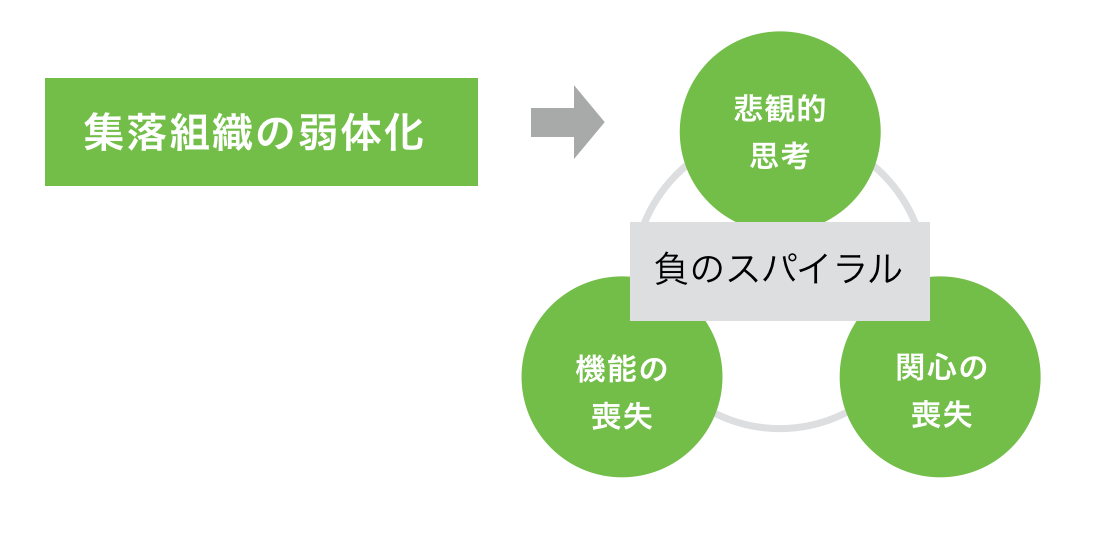
\includegraphics[width=1.0\hsize]{./images/17.png}
    \caption{過疎地域による負のスパイラル[5]}
    \label{fig:tmu_hino}
  \end{center}
\end{figure}




\subsection{本研究の目的}
筆者はこれまでに述べた背景を踏まえ,過疎地域の内発的な発展を推進するために必要不可欠である地域再生にむけた地域住民のモチベーションを高めるために,地域愛着とシビックプライドを育む「対話と交流の“場”」を形成する手法について考察する.「対話と交流の“場”」の詳細については2章で示す。そこで以下のように目的と達成手順を定義した。
\begin{itemize}
\item 研究目的 \\「対話と交流の“場”」形成によって過疎地域における地域コミュニティーを強化する.

\item 達成手順\\
\begin{enumerate}
\item 対話と交流の場の先行事例と地域活性化の概念の整理
\item 研究対象地域において行われたワークショップの考察
\item 過疎地域のためのガイドライン設定とパターン作成
\item ガイドラインの有効性の検証
\end{enumerate}

\end{itemize}

\subsection{本論文の構成}
本論文の構成を以下に示す.
\begin{itemize}
\item 第1章 序論  \\本研究の概要,背景と研究目的・達成用件について述べ,本論文の構成について説明する.
\item 第2章 先行研究と概念の整理  \\先行研究と概念の整理を行い,限界集落における地域活性化活動での本論文の位置付けを述べる.

\item 第3章 対象地域  \\本研究で実践の場として横根地区を選定した理由を述べ,地域住民の地域関心を図るためにアンケート調査・現地調査を行い,それらの結果から対象地域について詳述する.
\item 第4章 交流の“場”におけるガイドラインの設定 \\先行研究に基づき,ウェブサイト構築ワークショップについて検討し,「過疎地域の“場”の形成(手法)における設計・運営の指針を定め,「パターン」にまとめる.

\item 第5 章交流の“場”におけるガイドラインの有効性の検証 \\新潟県魚沼市横根集落において,第4章で設定した指針をもとに“場”の実践を行い,有効性の検証を行う.
\item 第6章 まとめ \\本研究の結論および研究成果が持つ意義を述べる.新たな問題点や展望をまとめる.


\end{itemize}
\newpage

\section{先行研究と概念の整理}
本章では,地域活性化の定義をした後,地域活性化活動と地域住民の主体性・愛着との関係性を既存の研究から明らかにする.さらに過疎地域における地域活性化活動での本論文の位置付けを述べる.
\subsection{地域活性化の定義}
地域活性化の定義は,担い手形成と生産動向に着目し地域農林業の活性化状況(農林業活性化度)を捉えた「農林業活性化」や各市町村の人口動態と人口構成に着目した「人口的活性化」など,複数ある.また国土交通省は、「経済的
要素、社会的要素、文化的要素、空間的要素」の4つの視点から地域活性化
を測ることが重要である\cite{kasseika}と整理している。つまり地域の資源や人口、環境をはじめとした様々な要素が絡み合うため、地域活性とは何なのかを定義するのは難しい。得に、過疎地域において考えた場合,条件が不利であることかた集落が人口減少にあるなかで,産業を生むことや,交流人口を単純に増やすことを考えるには破綻がある.そこで本研究では塩見\cite{shiomi}が提唱する「活性化とはそこに住む人びとが地域の資源を活用し,生きいきとした創造的な生活を営んでいる状態,またはそうした目標に向かって努力している状態を指すのであろう」という提唱を活性化の定義とする.\par
また,このような地域活性化を促す活動においては,地域への愛着が強い人ほど居住継続意識を示し地域活動へ積極的に参加する意識が高いことや,町内活動やまちづくり活動などの活動に熱心であること\cite{7}がわかっている.つまり,地域に対する地域活性化活動はその土地に対する愛着やシビックプライドが高いという二点が重要であり,これを高めるためには住民の主体性や地域当事者性を育んでいくことが必要となる.\par

\subsection{対話と交流の“場”}
“場”に関して,清水博は,一般に人々が身体を関与させながら共創的コミュニケーションをおこなう 「共創の舞台」 を “場”と呼び\cite{8},伊丹敬之は,“場”とは,「人々がそこに参加し,意識・無意識のうちに相互に観察し,コミュニケーションを行い, 相互に理解し,相互に働きかけ合い,相互に心理的刺激をする,その状況の枠組みのこと」 「人々の間の情報的相互作用と心理的相互作用の容れもの」 と定義している\cite{9}. さらに,和田宰は,「異なる価値観や能力を持つ『ひと』」 が,相互作用を通じて創造的な活動を生み出していくためには,『創発』を生み出す相互作用の場をつくることが不可欠である」 「場が与えられることによって,それぞれの『ひと』は潜在的な価値観や能力を顕在化させ,他の『ひと』との相互作用を通じて,創造的な活動を生み出す可能性を得ることになる」 と“場”の重要性を指摘している\cite{10}.つまり“場”とは、参加者同士が刺激しあいながら相互作用が生まれる空間のことである。その上で,まちづくりの展開における“場”について,久隆浩は,地域に暮らす人々が集まり,自由に意見交換や情報交換し,楽しく気軽に話を展開し,その中から,気づきが生まれ,新たなつながりが生まれていく「交流の場」の重要性を指摘している\cite{11}\par
これらの“場”の概念からもわかるように,地域活性化を促す活動においては,単に参加できる“場”の形成ではなく,対話や交流を通じて相互作用や関係変容が起こる “場”の形成が必要である. そうした“場”からつながりや輪が生まれ,活動や事業 (アクションやプログラム),組織が創発する. さらに,プロセスを通じてシビックプライド,市民の主体性や地域当事者性の育みが進み,新しい公共の創出につながっていくことが期待されるのである.\par
\subsection{“場”の形成手法}
とはいえ、ただ単純にひとが集まる“場”をつくれば,自動的に相互作用や関係変容が起こり,何かが生まれるというわけではない.世田谷まちづくりセンターは,参加のデザインとして,①プロセスデザイン, ②プログラムデザイン,③参加形態のデザインの三つのデザインを挙げている\cite{12}\par.さらに世古一穂は,①参加のプロセスデザイン,②参加のプログラムデザイン,③参加構成のデザインの三つのデザインの重要性を挙げている.\cite{13}\par状況に応じて,どのように場をデザインしていくのか,どのように運営していくのかという場づくりの方法が問われているといえる.\par
このように,“場”の形成手法については,複数の調査・研究がされてきた一方で、過疎集落における地域活性化を目的に実践した例はない.そこで本研究ではこの点に着目し,第1章で述べたように、過疎地域において必要とされている地域主体性とシビックプライドを向上させる「対話と交流の“場”」を形成する手法について考察する.\par
\subsection{パターン・ランゲージ}
“場”の形成におけるファシリテートやプログラムデザインは,経験値が重要であり,成功の“秘訣“ともいうべきものは,「実践知」「暗黙知」「センス」「勘」「コツ」などといわれなかなか他者には共有しにくい.そこで本研究では,成功事例の中で繰り返し見られる「パターン」を抽出し,抽象化を経て言語(ランゲージ)化することでノウハウを持つ個人がどのような視点で,どんなことを考えて,何をしているのかを,他の人と共有可能であるパタン・ランゲージ手法\cite{ptn}を参考に,“場”の形成手法の確率を目指す.\par
パターンランゲージ手法とは、1970年代に建築家クリストファー・アレグザンダーが住民参加のまちづくりのために提唱した知識記述の方法であり、町や建物に繰り返し現れる関係性を「パターン」と呼び、それを「ランゲージ」(言語)として共有するために考案されたものである。\cite{arek}建築分野で発展したパターン・ランゲージは、1990年代にソフトウェアの分野に取り入れられ、2000年以降は人間の行為の秘訣を記述するために応用されるようになった。図◉の例からも分かる通りパターンは、デザインにおける「問題」と、その「解決」の発想が一対となって記述され、それに名前が付けられる。パターン・ランゲージの利用者には、自らの状況に応じてパターンを選び、そこに記述されている抽象的な解決方法を、自分なりに具体化して実践することが求められる。一定の記述形式で秘訣を記することによって、パターン名に多くの意味が含まれ、それが共通で認識され、「言葉」として機能するようになるのである。\cite{ptn}


\begin{figure}[H]
  \begin{center}
    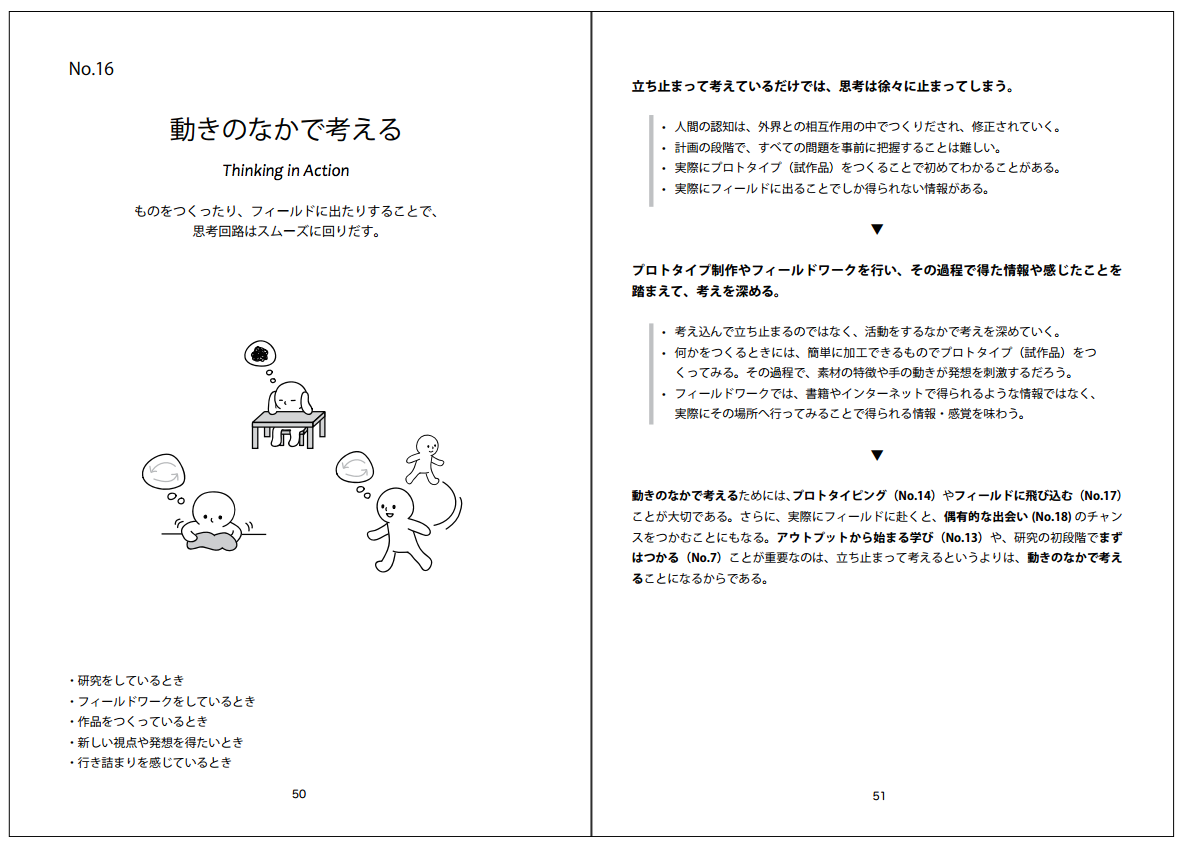
\includegraphics[width=1.0\hsize]{./images/ptn.jpg}
    \caption{学習パターン(Learning patterns)-\cite{ptn}より参照}
    \label{fig:tmu_hino}
  \end{center}
\end{figure}


\newpage
\section{対象地域}
本研究で実践の場として横根地区を選定した理由を述べ,アンケート調査・現地調査をもとに対象地域について詳述する.
\subsection{地域の概要}
本研究の対象地として,新潟県魚沼市横根地区を対象を選定した.筆者の所属する研究室が,平成26年7月より3月まで新潟県により大学生の力を活かした集落活性化事業の助成を受けている点,人口や高齢化率の規模が一般的な過疎地域と同等と言え本研究の対象に合致する点を考慮する.\par
この地区が位置する新潟県中越地方の南部に位置する魚沼市は,水や気候がコシヒカリの栽培に最も適していると言われ,米の名産地として知られている.2016年月現在の推計人口は約3万7千人である.\par
図2に示したように、横根地区は魚沼市北部にあり、中心市街地から車で40分の場所に位置する。日本海気象地区に属す典型的な豪雪地帯であり,通年積雪3mにも及び,根雪日数は130日以上となっている.横根地区の地域資源としては,稲作があげられ,地域の7割以上の世帯が兼業ではあるが稲作を営んでいる.さらに市が運営する越後ハーブ香園入広瀬が集落の山頂に位置している.都市部からのアクセス条件は良いとは言えず,離村した若年層が頻繁に帰省できる距離ではない.\par
2016年4月時点の推計人口は113人,世帯数は52世帯,高齢化率46.9%であり、図3からもわかるように、地域のほとんどが50代以上で構成されており、15歳から25歳の青年世代は存在しない。近年、30代の母親世代が地域にUターンしたことにより、子供が地域にふえたが、5年前までは30代以下がひとりもいない時期が続いていた。\par
平成26年より総務省による地域力の創造・地方の再生の一環で「地域見守り」のための地域おこし協力隊の派遣を受けている.
\begin{figure}[H]
  \begin{center}
    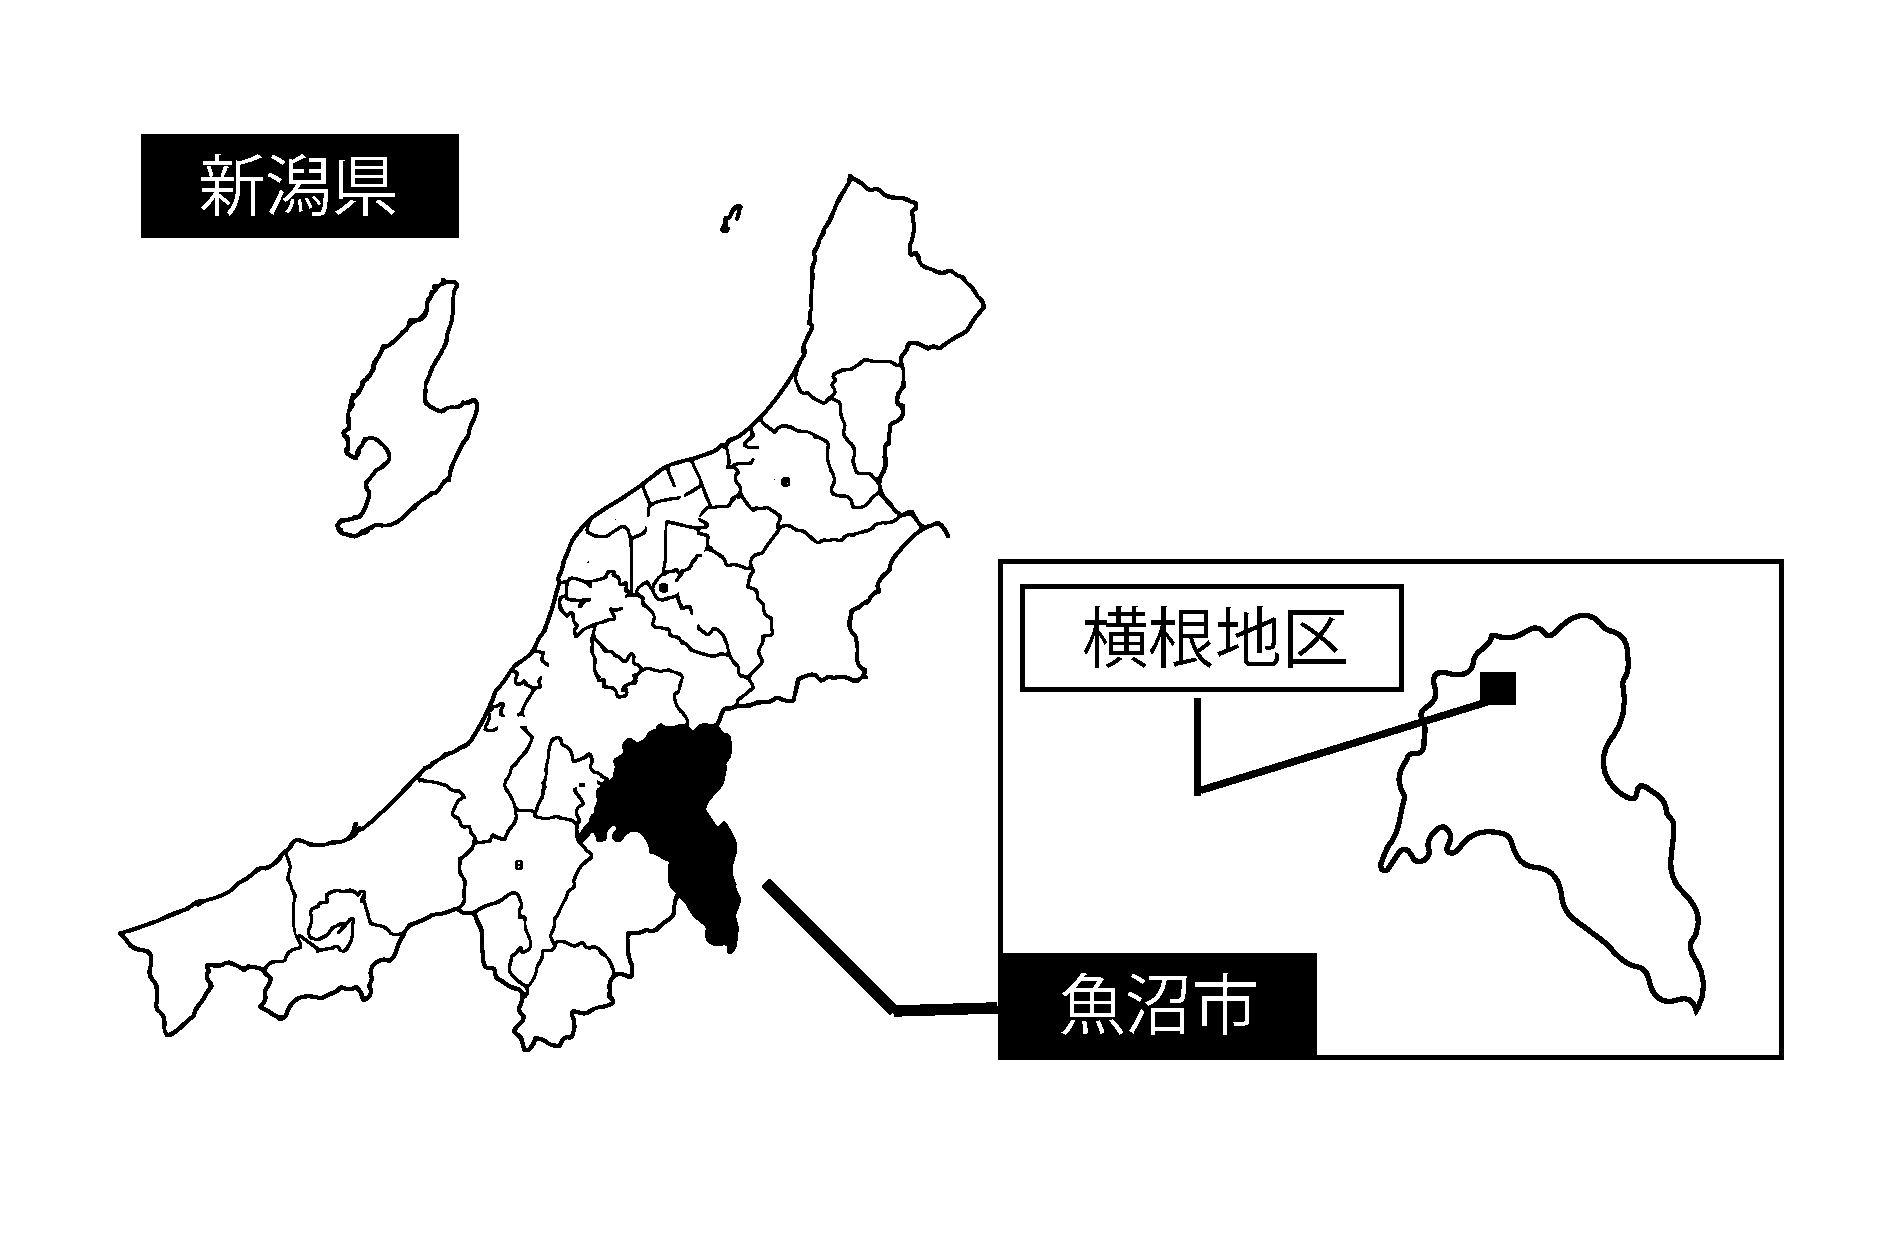
\includegraphics[width=1.0\hsize]{./images/yokone_place.pdf}
    \caption{魚沼市における横根集落の位置}
    \label{fig:tmu_hino}
  \end{center}
\end{figure}
\begin{figure}[H]
  \begin{center}
    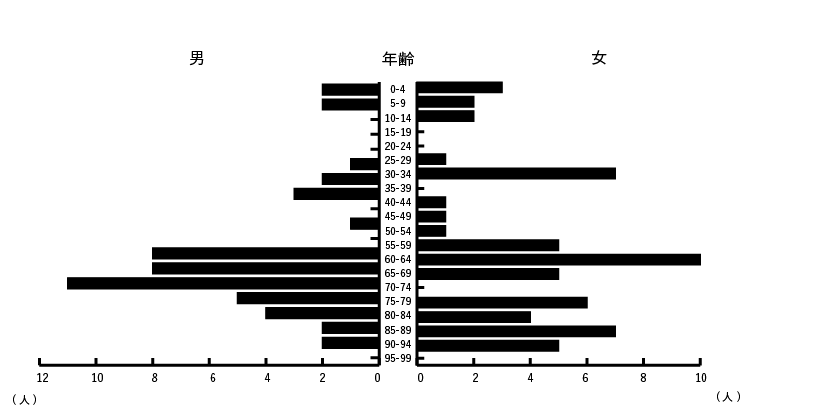
\includegraphics[width=1.0\hsize]{./images/zinnkou.jpg}
    \caption{横根地区の世代別人口統計(平成28年)}
    \label{fig:tmu_hino}
  \end{center}
\end{figure}

\subsection{現地調査の実施}
横根地区の資料収集,地域資源の把握,現地住民への聞き取りなどを行うため、長期滞在も含め定期的に計9回集落を訪問し、現地調査を行った。(図4)

\begin{figure}[H]
  \begin{center}
    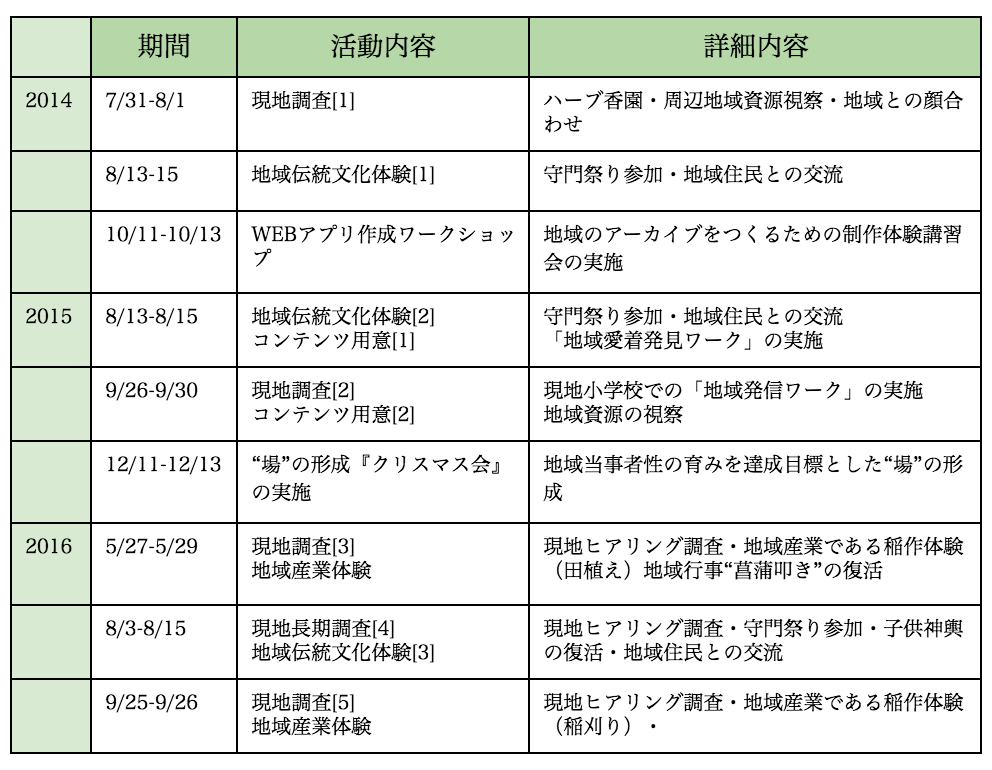
\includegraphics[width=1.0\hsize]{./images/18.png}
    \caption{現地活動スケジュール}
    \label{fig:tmu_hino}
  \end{center}
\end{figure}
2014年7月に行われた初回現地調査時に、住民アンケート調査を行った。回答者は22名である。「地域に対しての気持ちをおしえてください」の質問において,図
5で示した通り、すごく嫌いーすごく好きまでの7段階評価で平均が5.8となり,自分の地域への愛着度が比較的高いことがわかった.しかし,ヒアリングからは「こんなところにひとなんかこない。」「自分の生まれ育った地域だから愛着はあるけれど,できるなら出て行きたい。」などといった地域に対して後ろ向きな発言が多く聞かれ,シビックプライドが低いことがわかった.

\begin{figure}[H]
  \begin{center}
    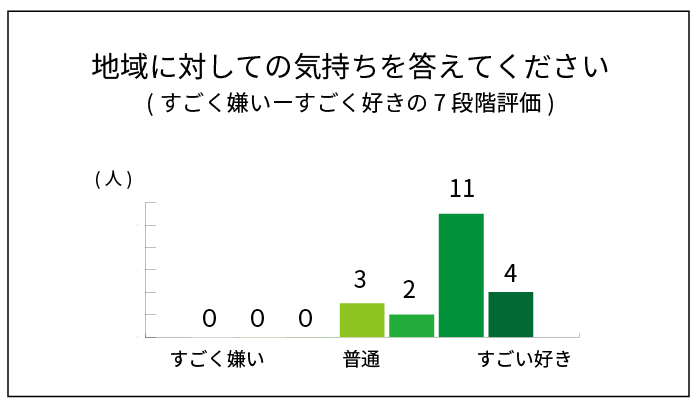
\includegraphics[width=1.0\hsize]{./images/03.png}
    \caption{アンケート調査1(地域への愛着意識調査)}
    \label{fig:tmu_hino}
  \end{center}
\end{figure}
\begin{figure}[H]
  \begin{center}
    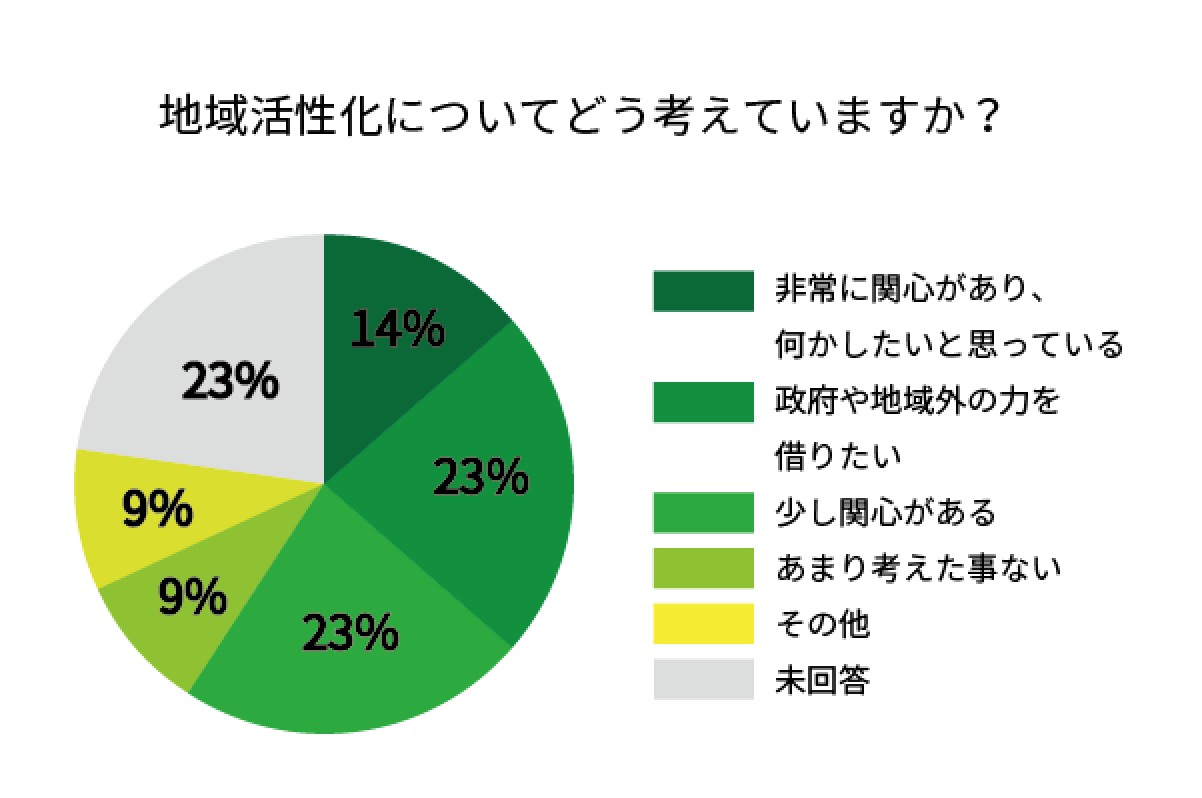
\includegraphics[width=1.0\hsize]{./images/02.png}
    \caption{アンケート調査1(地域活性化に関する意識調査)}
    \label{fig:tmu_hino}
  \end{center}
\end{figure}
「地域活性化についてどう考えていますか?」の質問では、図6の通り地域の今後を考える地域活性化活動にについては,問題意識をもっているひとは大半を占めているにもかかわらず,自分で行動しようという主体性を持っている人は,全体の2割にも満たないことがわかった.\par
地域には「役員会」と呼ばれる自治組織が存在しており,地域の決まりごとや大きな経費がかかるものに対して会議を行い,地域運営を行っていく10名ほどの集団が存在している.以前は他にも「子供会」,26歳から30歳の青年が集まり体育祭やレクリエーション,消防団の指導を行う「青年団」,花見や温泉旅行を行う「婦人会」,65歳になると入会する「老人会」などの『年齢集団』.さらに,消防練習を行う「消防団」や毎年行われる守門神社の祭りの運営を行う「祭り実行委員会」,農協や役場との農業の総括を行う「農業組合」などの『機能集団』が存在していたが,現在は人口の減少とともに形骸化し,現在は実質的にすべての自治組織の構成員と役割が同一化している.このため,世代ごとの連体感や世代を超えたコミュニケーションが減ってきているといえる.\par
地域のヒアリング調査からも,昔は毎年やっていた子供神輿などの地域行事や集まりが徐々に減少し,住民同士が世代・性別に関係なく集まる機会が減ってきているということがわかった.

\newpage
\section{交流の“場”におけるガイドラインの設定}
2014年度に対象地域で実施したウェブサイト構築ワークショップについて、世古一穂らの「参加と協働のデザイン」\cite{13}に基づき検討し,不満点を解決するために,過疎地域の“場”の形成における設計・運営のガイドラインを定め,「パターン」にまとめる.
\subsection{ウェブサイト構築ワークショップ}
対話と交流の場づくりの一手法として「地域の問題を多くの住民がそれぞれの年齢や社会的な立場にとらわれることなく, 水平的な関係で話し合い, 創造的自己解決していくための場」\cite{14}として「ワークショップ手法」が様々な場面で広く使われ,具体的な成果も出ている. その点から,2014年に対象地域で菊本\cite{15}を中心に行ったウェブサイト構築ワークショップを「対話と交流の“場”づくり」の観点から考察する.
\subsubsection{概要}
2014年10月12日,横根集落内にあるみずほ会館において,地域の魅力を発信するWEBアプリ作成のためのマッピングワークショップを行った.参加者は図8の通り、集落在住の50代から70代の男性9名,女性1名、計10名となった.運営は研究室メンバー6名,外部協力者1名の計6名で行う.紙地図を使用した作業と,ウェブ構築作業の二部構成でおこなった.手順は以下の通りである.なお,告知時に参加者には横根集落で撮影された写真を持参するように依頼している.\\
\begin{enumerate}
\item  … 事前に制作したデモ版を元にした最終イメージの共有.
\item  … 集落の地図を1.5[m]×2[m]の紙地図に印刷し,それを囲みながら持参した写真の撮影場所,撮影時期,当時の状況を話しあう.
\item … 特定されたら,紙地図上の撮影場所に写真をマスキングテープで貼付する.また,時期や状況はポストイットに記入し,写真に貼付する.

\item  … データ作成の担当を決定する.

\item …マッピングシステムを利用し,写真データに位置情報,撮影年代,撮影者,状況などを付与する.
\item …成果物観覧
\end{enumerate}
\subsubsection{考察}
世古一穂らの「参加と協働のデザイン」」\cite{13}より,1)場の運営,2)個々の場の位置づけ, 3)場の設計の三点から,ワークショップを検討する.\\
\begin{enumerate}
\item 場の運営\\
テーマを,『地域のアーカイブをつくるための制作体験講習会』とし,紙地図を使用した作業と,ウェブ構築作業の二部構成で行った.世古ら\cite{13}は交流の“場”づくりにおいて,「ファシリテーション」 を通じて特定のゴールに誘導していくことではなく,状況に対して,しなやかで,かつ,柔軟に対応していくことが求められていると明記している.しかし,地域活動に対して意欲がある人が集まっているわけではない過疎集落の状況で今回のような制作物が決まっている講習会形式でテーマ設定を行うと,プロセスを通じて方向性・枠組み,目的・目標自身が変化していくことに柔軟に対応することが難しく,「やらされている感」「よくわからない感」を感じている参加者がでてきてしまった.あらかじめ明確な目標を設定した上で話し合いを行うことよりは,対話や交流を通じてアクションが創出されることを期待した場づくりが有効であると考えられる.\\
\item  個々の場の位置づけ\\
横根地区では、地域の主な情報伝達を地区を5つに分けて回す回覧板を使用して行われる。そこでワークショップの告知は,回覧板に挟むチラシ(図7)を用意して行った。その結果,図8の通り、参加した住民は50代から70代の男性であり,全員当時の地域自治組織の構成員であることがわかった。地域自治組織の構成員は普段から,共同体意識が強く,“決まりであるから”,“集落のためになるから”という理由で集まりに参加する意識がある.その一方で,地域に古くからある地域行事の中心は家長である男性が代表となって行うという慣習から,女性が地域活動に積極的に参加しにくいということもその後のヒアリングから分かった.とくに,地域には出身者の若い母親が何人かいるが,地域活動にはあまり前向きではなく,「男の人がいくもの」「自分たちのでる幕でない」といおもっていることがヒアリングから聞こえてきた.場を形成する際には,全体の枠組みから見て個々の場の位置づけがどのような視点で,どのようにおこなわれているのかを明確にしておく必要がある.\\
\begin{figure}[H]
  \begin{center}
    \includegraphics[width=0.8\hsize]{./images/10.png}
    \caption{横根集落配布告知用フライヤー}
    \label{fig:tmu_hino}
  \end{center}
\end{figure}
\begin{figure}[H]
  \begin{center}
    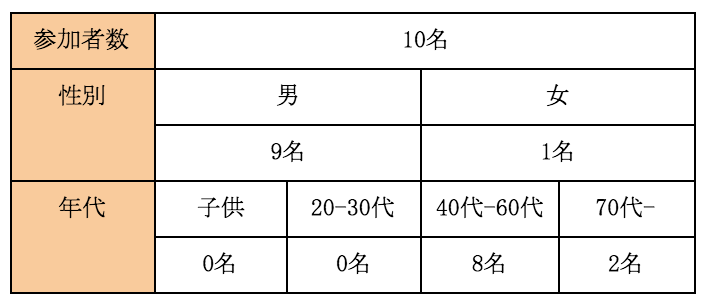
\includegraphics[width=0.6\hsize]{./images/19.png}
    \caption{参加者の属性}
    \label{fig:tmu_hino}
  \end{center}
\end{figure}

\item 場の設計\\
久隆によると,交流の場の運用上の課題として,参加者の主体性・自発性・自律性によって活動が展開されること, 他者に対して活動を強制しないこと,個人の資格で参加すること,多様な主体が参加することを挙げている.\cite{16}\par
紙地図作業では,図9でみられるように「この写真は〇〇にきけばわかるかな」「〇〇さんならくわしいかもしれない」「これは俺らが何歳の時かな〜」などと自発的に写真や地図を介して地域住民同士でのコミュニケーションが多く取られているのをみることができた. さらに図10の写真からわかる通り、左の青のジャンバーを来た学生スタッフに対して,「この時代はこんなだったんだよ」「これが俺だなあ。わかるか?」などと,当時の状況を詳しく話す場面も見られた. その一方でウェブ構築作業については,「難しい」「わからない」などの意見が多く聞かれ,全ての作業工程をスクリーンショットと説明とともにおさめた手順書やマッピングシステムなどを作成して,参加者のハードルをさげようと試みたが,「わかんないからやってくれー」などという声も聞かれ、技術のハードルが参加者の主体性を削いでしまっている点が課題として見えた.その後のヒアリングでも自分が制作に携わったという当事者意識は芽生えておらず,「なんかむずかしかった」「よくわからなかった」などという意見が多かった。\par
久隆の課題から見て、多様な主体が主体的に参加するとともに、その様々な世代が主体性・自発性・自律性によって自然と交流できる“場”を形成する仕組みが必要があると考えられる.\par

\begin{figure}[H]
  \begin{center}
    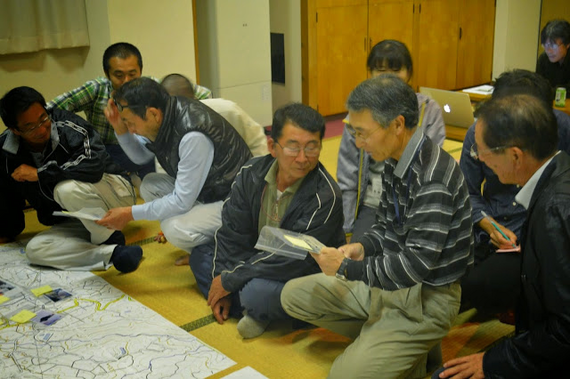
\includegraphics[width=0.8\hsize]{./images/komenoma-2.png}
    \caption{紙地図作業1(世代間交流の様子)}
    \label{fig:tmu_hino}
  \end{center}
\end{figure}
\begin{figure}[H]
  \begin{center}
    \includegraphics[width=0.8\hsize]{./images/DSC_0054.JPG}
    \caption{紙地図作業2(スタッフへの地域がたりの様子)}
    \label{fig:tmu_hino}
  \end{center}
\end{figure}

\end{enumerate}
これらの検討から,過疎地域の“場”の形成における大きな課題として「参加者の世代・性別のばらつき」,当事者意識の低い地域住民に対する「地域活動へのハードル」があげられることがわかった.



\subsection{過疎地域における交流の“場”におけるガイドライン}

これらの課題を解決するために,1)場の運営,2)個々の場の位置づけ, 3)場の設計の枠組みにおいて,過疎地域の“場”の形成における設計・運営のガイドラインを定め,「パターン」にまとめる.\\\\
\begin{enumerate}
\item 
\textbf{場の運営…『場の運営柔軟な枠組みに基づいた運営や進行』}\\
1-A:[目的におかない目標] :枠組みをもったアウトプット重視よりも対話や交流による創発性を通じた空間を重視する.\\\\
地域活動を目的にした“場”の形成において,最終的に評価されるのは「結果」であるため,それを生み出す「プロセス」には目が行きにくく,継続性や当事者性が低い
成果物や意思決定が生まれてしまいがちである.そこでまずは地域活動を目的におかず,目標として捉え対話や交流を通じた相互作用や関係変容を大事にする. プログラムはあるが, 必ずしもプログラム通りに実施するのではなく, 状況に応じた柔らかなマネジメントを心がける. フレーム (枠組み) も状況に応じて,再構成し, ゴール自身も変化させる. さらに話し合いが単に楽しかっただけに留まらず, 次に前向きな展開になるように心がけるようにする.\\\\

\item 
\textbf{個々の場の位置づけ…『多様な世代が参加しやすいプロセス』}\\
2-A:[目線の多角化]:過疎地域の慣習上,“場”に参加しづらい世代に,参加に際して具体的な役割を付与する.\\\\
過疎地域の地域住民はそれぞれ違うことに関心を持っており, 地域活動への関わり方の慣習も異なる. 特に当事者意識が低い世代に対して,まず参加してもらうことが第一の課題である.そこで,まずは地域活動の文脈に限らず世代ごとにその世代にあった“場”における役割を担ってもらうことで参加のハードルを下げるようにする.一つの“場”っであっても様々な目線があることを意識する.\\\\

2-B:[伝達の最適化]:各世代に適した情報伝達の方法を用いて,“場”への参加を呼び掛ける.\\\\
従来おこなわれている回覧板での情報伝達だけではなく,各世代に適した情報伝達の方法を使い分けるようににする.世代ごとの呼びかけ方も考慮する.\\\\


\item
\textbf{場の設計…『参加者の想いや関心を自然に引き出す場づくり』}\\
3-A:[起爆のための仕込み]:事前に地域住民の意見を集め,フラットに表現するコンテンツを用意し,会話を促進する.\\\\

人口の減少とともに対話や交流が減ってきた過疎地域において,自発的に地域活性のための対話や交流が生まれることは難しい.そこでWEBアプリ作成のためのマッピングワークショップの写真を使った紙地図作業を参考にし,会話を促すための起爆剤となるコンテンツを用意する.参加者が身近に感じられるように,地域関係者が関係した資料を収集,編集する.\\\\

3-B:[協働作業]:様々な年代のメンバーが参加するチームを編成し,世代を超えた協働作業を行なう.\\\\
ただ“場”を用意したところで,同じ世代や親戚,関わりが多くある人とばかり話がちになってしまう.普段関わることの少ない世代や性別同士をあえて混ぜたグループを作り,協働作業を行うことでより新しい相互作用や関係変容が期待できる.\\\\
3-C:[自然体]:開催する場所・時間帯を,地域の慣習に合わせることにより,メンバーが気張らず,平常心で参加できるようにする.\\\\
改めて“場”ということを意識し強調してしまうと,縮こまり緊張してしまい,会話が弾まない.フラットな関係性でお互いが自然体で参加できるように地域の慣習をヒアリングし“場”の設計を考慮する.
\\\\
\end{enumerate}

\newpage
\section{交流の“場”作りにおけるガイドラインの検証}
新潟県魚沼し横根集落において,本研究で設定したガイドラインの軸に作成した幾つかのパターンを元に今回の“場”作りを実践・考察し,ガイドラインの有効性の検証を行う.

\subsection{概要}
2015年12月12日,横根集落内にあるみずほ会館において,どの年代でも気軽に参加できる“クリスマス会”をテーマに定め,ガイドラインに沿って,“場”の形成を行う.話題促進コンテンツは,事前にお祭りでのインタビュー,小学校でのワークショップを行い,用意する.参加者は集落在住の50代から70代の男性7名と女性4名,30代女性5名,子供7名 計23名となった.運営は研究室メンバー5名,外部協力者1名の計6名で行った.準備段階を含め,プログラムは以下の通りである.\\

\begin{enumerate}
\item  … 開催準備\\
 ・プレゼントオーナメント作り\\
 ・食事づくり
\item  … チームわけ
\item … チームで力を合わせて行う,紙飛行機の飛行距離を競うゲーム
\item  … チームそれぞれのクリスマスケーキ作成
\item …食事(コンテンツ鑑賞)
\item …子供達によるクリスマスプレゼントの配布\\
\end{enumerate}



\subsection{ガイドラインの適用}
\subsubsection{場の運営柔軟な枠組みに基づいた運営や進行}\\
1-A:[目的におかない目標] :枠組みをもったアウトプット重視よりも対話や交流による創発性を通じた空間を重視する.\\\\
テーマをどの年代でも気軽に参加できる「クリスマス会」に設定した.シビックプライド,地域当事者性の育みは主催者側が掲げる達成目標とし,参加者には明かさずに,地域の様々な世代があつまり楽しむ“場”としての役割を押し出すことにより,自由な空間を意識した.\\\\

\subsubsection{多様な世代が参加しやすいプロセス}
2-A:[目線の多角化]:過疎地域の慣習上,“場”に参加しづらい世代に,参加に際して具体的な役割を付与する.\\\\
参加するハードルを下げるため,「開催のお手伝いをお願いしたい.」という呼びかけを行い,子供たちには「地域住民へのプレゼント作り」を,若い世代の女性には「料理の準備」高齢者の女性には「料理の準備の補佐」をそれぞれ,役割として担ってもらった.\\\\


2-B:[伝達の最適化]:各世代に適した情報伝達の方法を用いて,“場”への参加を呼び掛ける.\\\\
通常の回覧板での呼びかけ(図11)・地域協力者の呼びかけにプラスして,若い世代にはコミュニケーションアプリLINEを活用し,グループを作成して呼びかけを行った.同様のグループを使用し,子供達にも,母親からの伝達で呼びかけを行った.
\begin{figure}[H]
  \begin{center}
    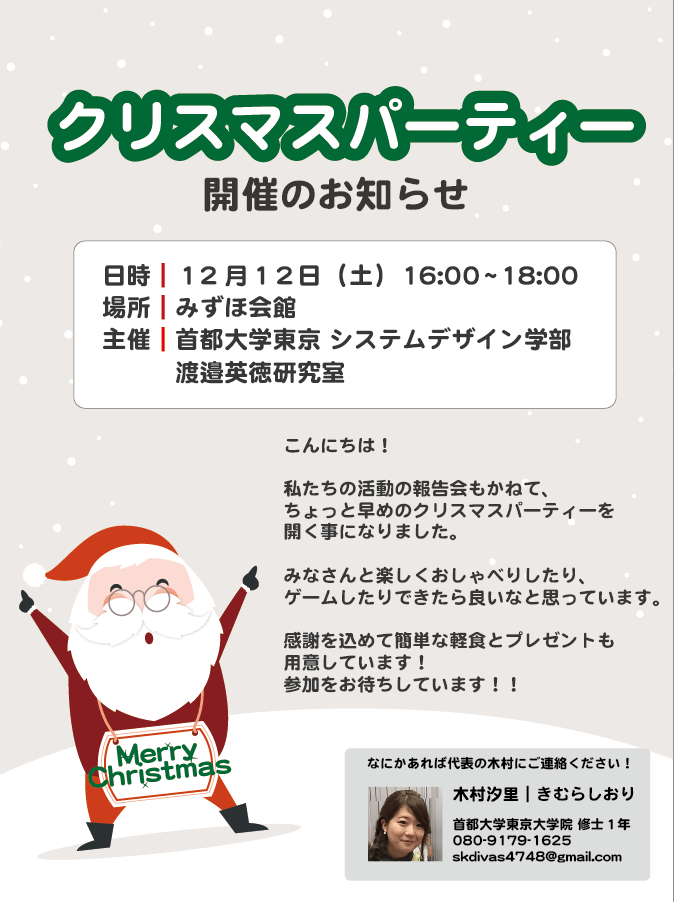
\includegraphics[width=0.8\hsize]{./images/05.png}
    \caption{横根地区回覧用告知フライヤー}
    \label{chirstmas2}
  \end{center}
\end{figure}

\subsubsection{参加者の想いや関心を自然に引き出す場づくり}\\
3-A:[起爆のための仕込み]:事前に地域住民の意見を集め,フラットに表現するコンテンツを用意し,会話を促進する.\\\\
パターン3-Aである[起爆のための仕込み]の会話促進コンテンツを制作するため,事前準備として事前に二つのワークを行った.地域住民・その関係者がコンテンツに参加していることが条件である.\\\\

\begin{itemize}


\subsubsubsection ◉ お祭りにおける地域愛,再確認ワーク\\
2015年8月16日に行われた横根地区地域行事であるの守門祭りを利用し,地域愛,再確認ワークを行った.守門祭りは,毎年1回行われ,地域外から帰省した出身者も集まる地区の伝統行事である.「横根の好きなところはどこですか?」の質問をお祭りの参加者に投げかけ,動画を撮影する.図◉で示した通り、在住が地域内外関わらず様々な世代の意見を聞くことができた。図◉からもわかる通り「いいところなんてないんだよなあ〜」といいながら質問の答えを一緒にお祭りにきた孫や親戚と一緒に周りの人とうれしそうに話し合っている町民の姿が印象的であった.さらに図◉が示す通り、個々の目線から様々な地域の良いところを抽出することができた。これらを一本の動画に編集する。

\begin{figure}[H]
  \begin{center}
    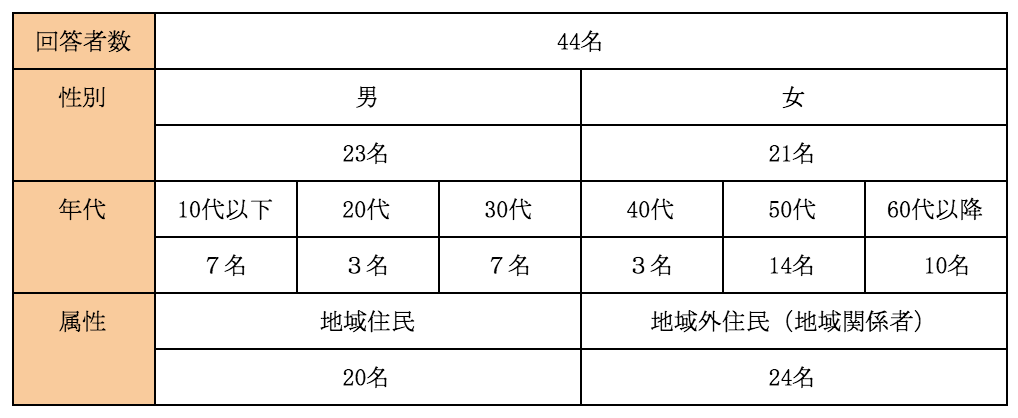
\includegraphics[width=0.8\hsize]{./images/21.png}
    \caption{回答者属性}
    \label{fig:tmu_hino}
  \end{center}
\end{figure}

\begin{figure}[H]
  \begin{center}
    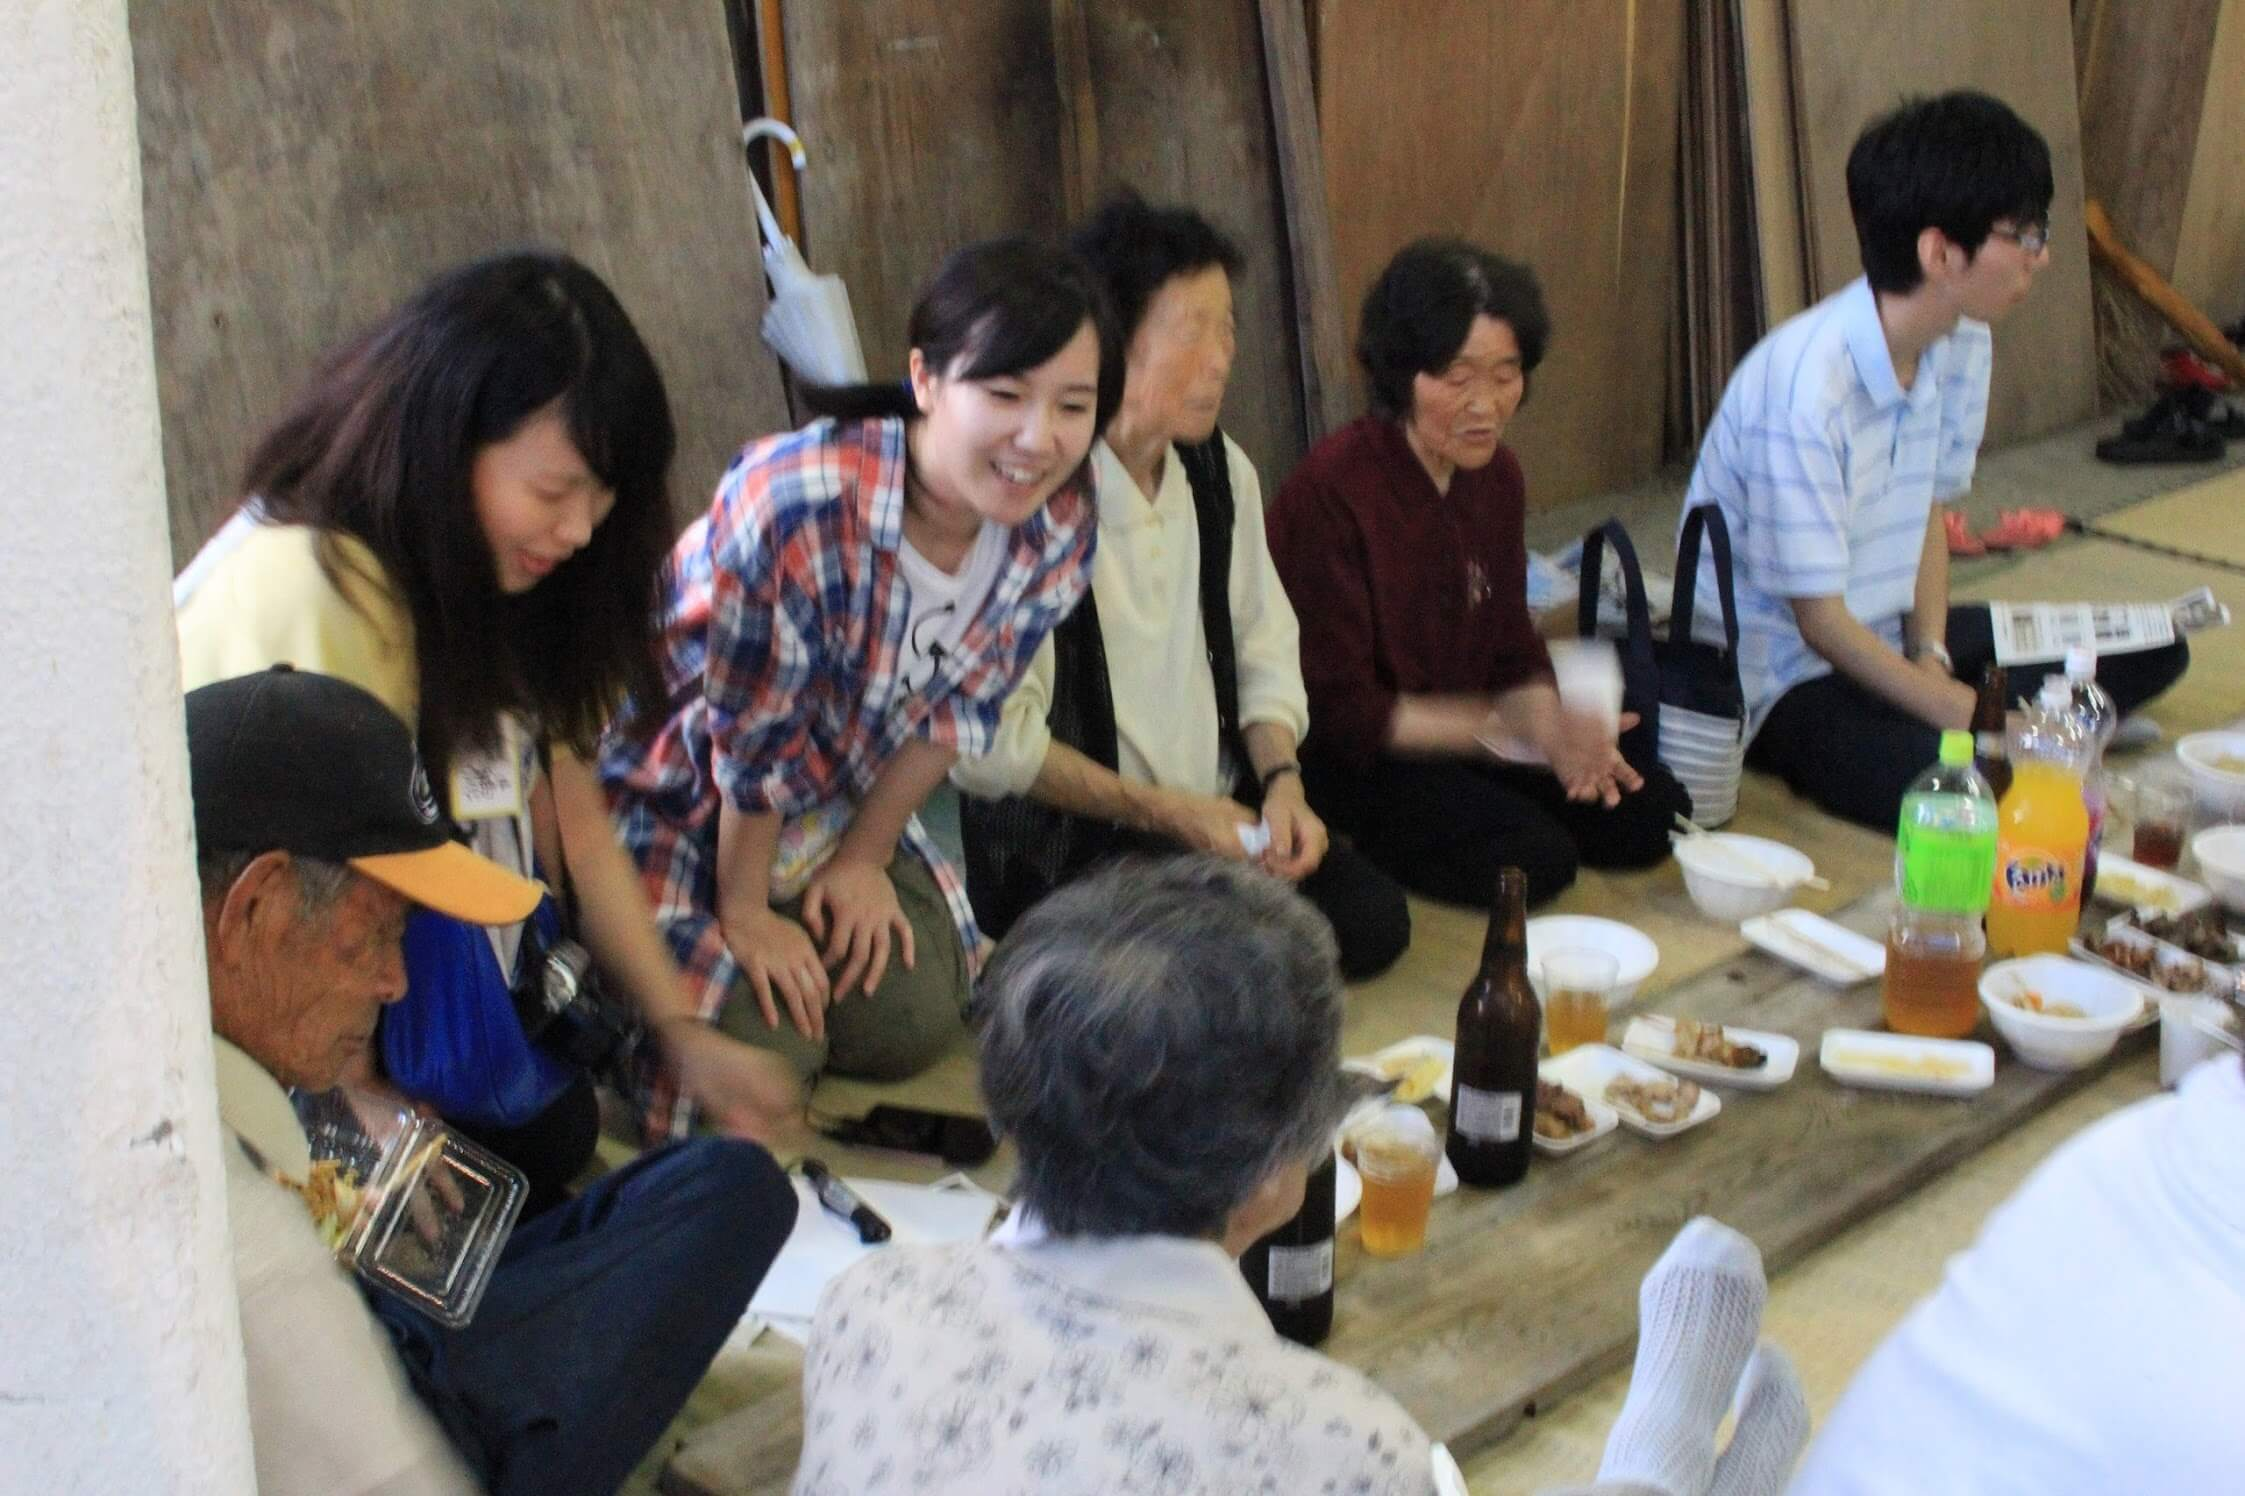
\includegraphics[width=0.8\hsize]{./images/IMG_4784.JPG}
    \caption{ワークの様子(メンバーへの地域語りの様子)}
    \label{fig:tmu_hino}
  \end{center}
\end{figure}
\begin{figure}[H]
  \begin{center}
    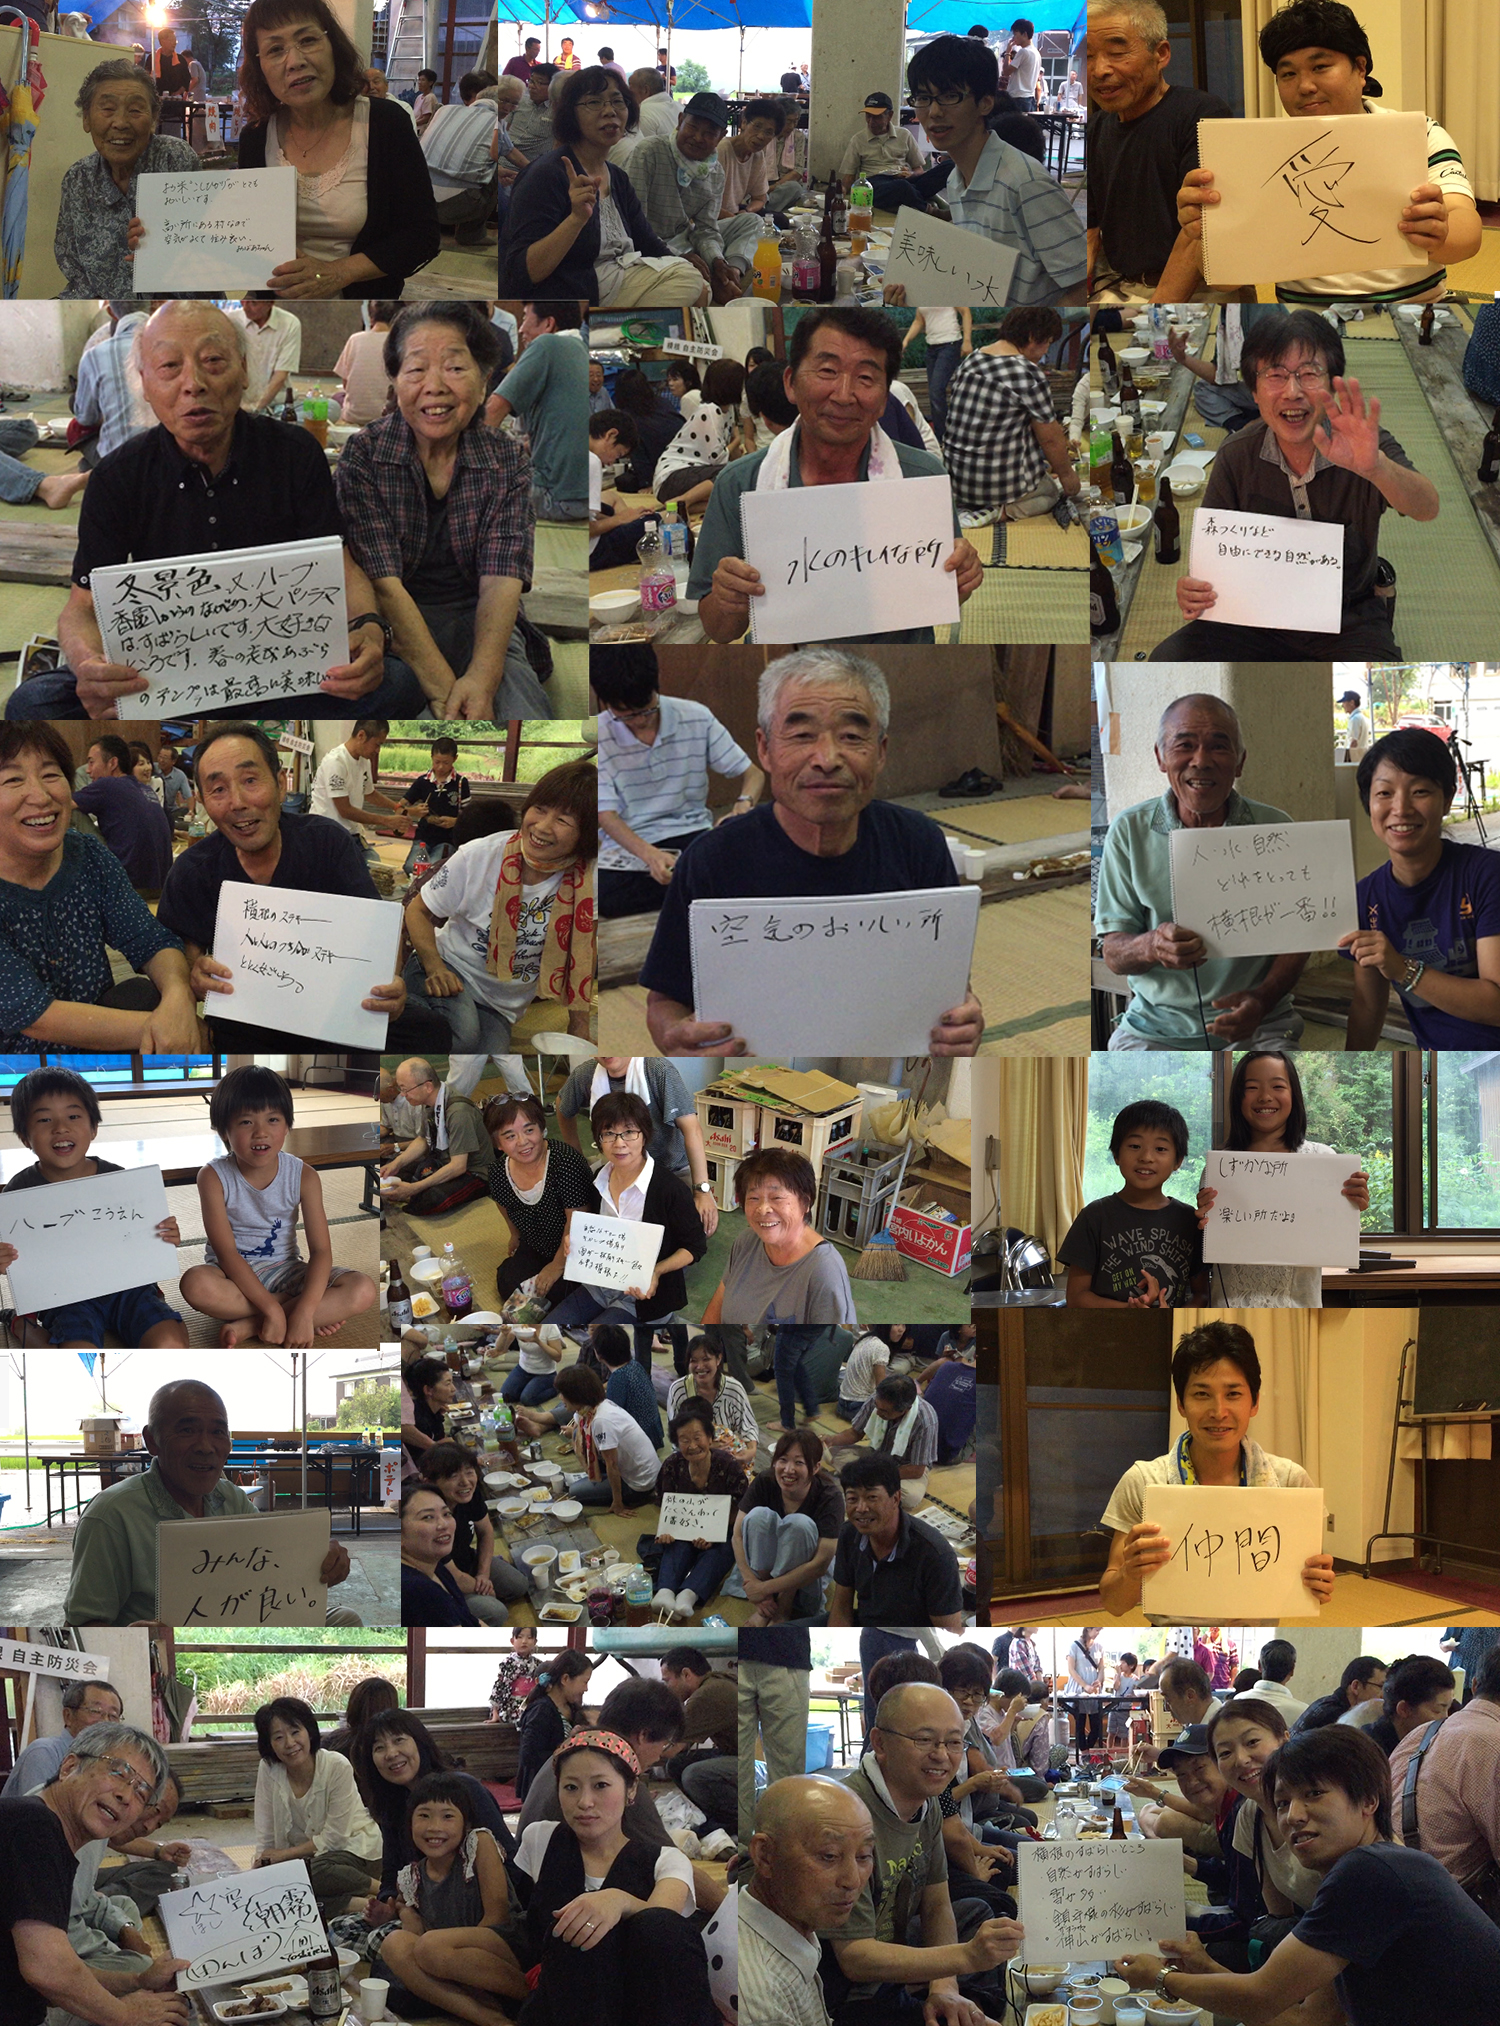
\includegraphics[width=1.0\hsize]{./images/yokone.jpg}
    \caption{成果物1}
    \label{fig:tmu_hino}
  \end{center}
\end{figure}


\subsubsubsection ◉ 小学校における子供たちによる地域発信ワーク\\
2015年9月16日に集落から車で20分の位置にある魚沼市立須原小学校の小学一年生と二年生の31名を対象に地域発信ワークを行った.この小学校は以前から集落にある越後ハーブ香園入広瀬を中心とした現地でのまちあるき課外授業を行っている.「ハーブこうえんをせかいにはっしんしよう!」をテーマにみんなが好きになったハーブ香園のものや場所か,自分たちが大人になる20年後のハーブ香園を想像してポスターに描いてもらうワークを行った。図◉の写真からもわかるように20年後には,ローカル線の只見線が停車する駅ができていたり,ツリーハウスが革新的な形になっていたり,子どもならではの未来への希望が一つ一つの絵に出ているのが印象的であった.

\begin{figure}[H]
  \begin{center}
    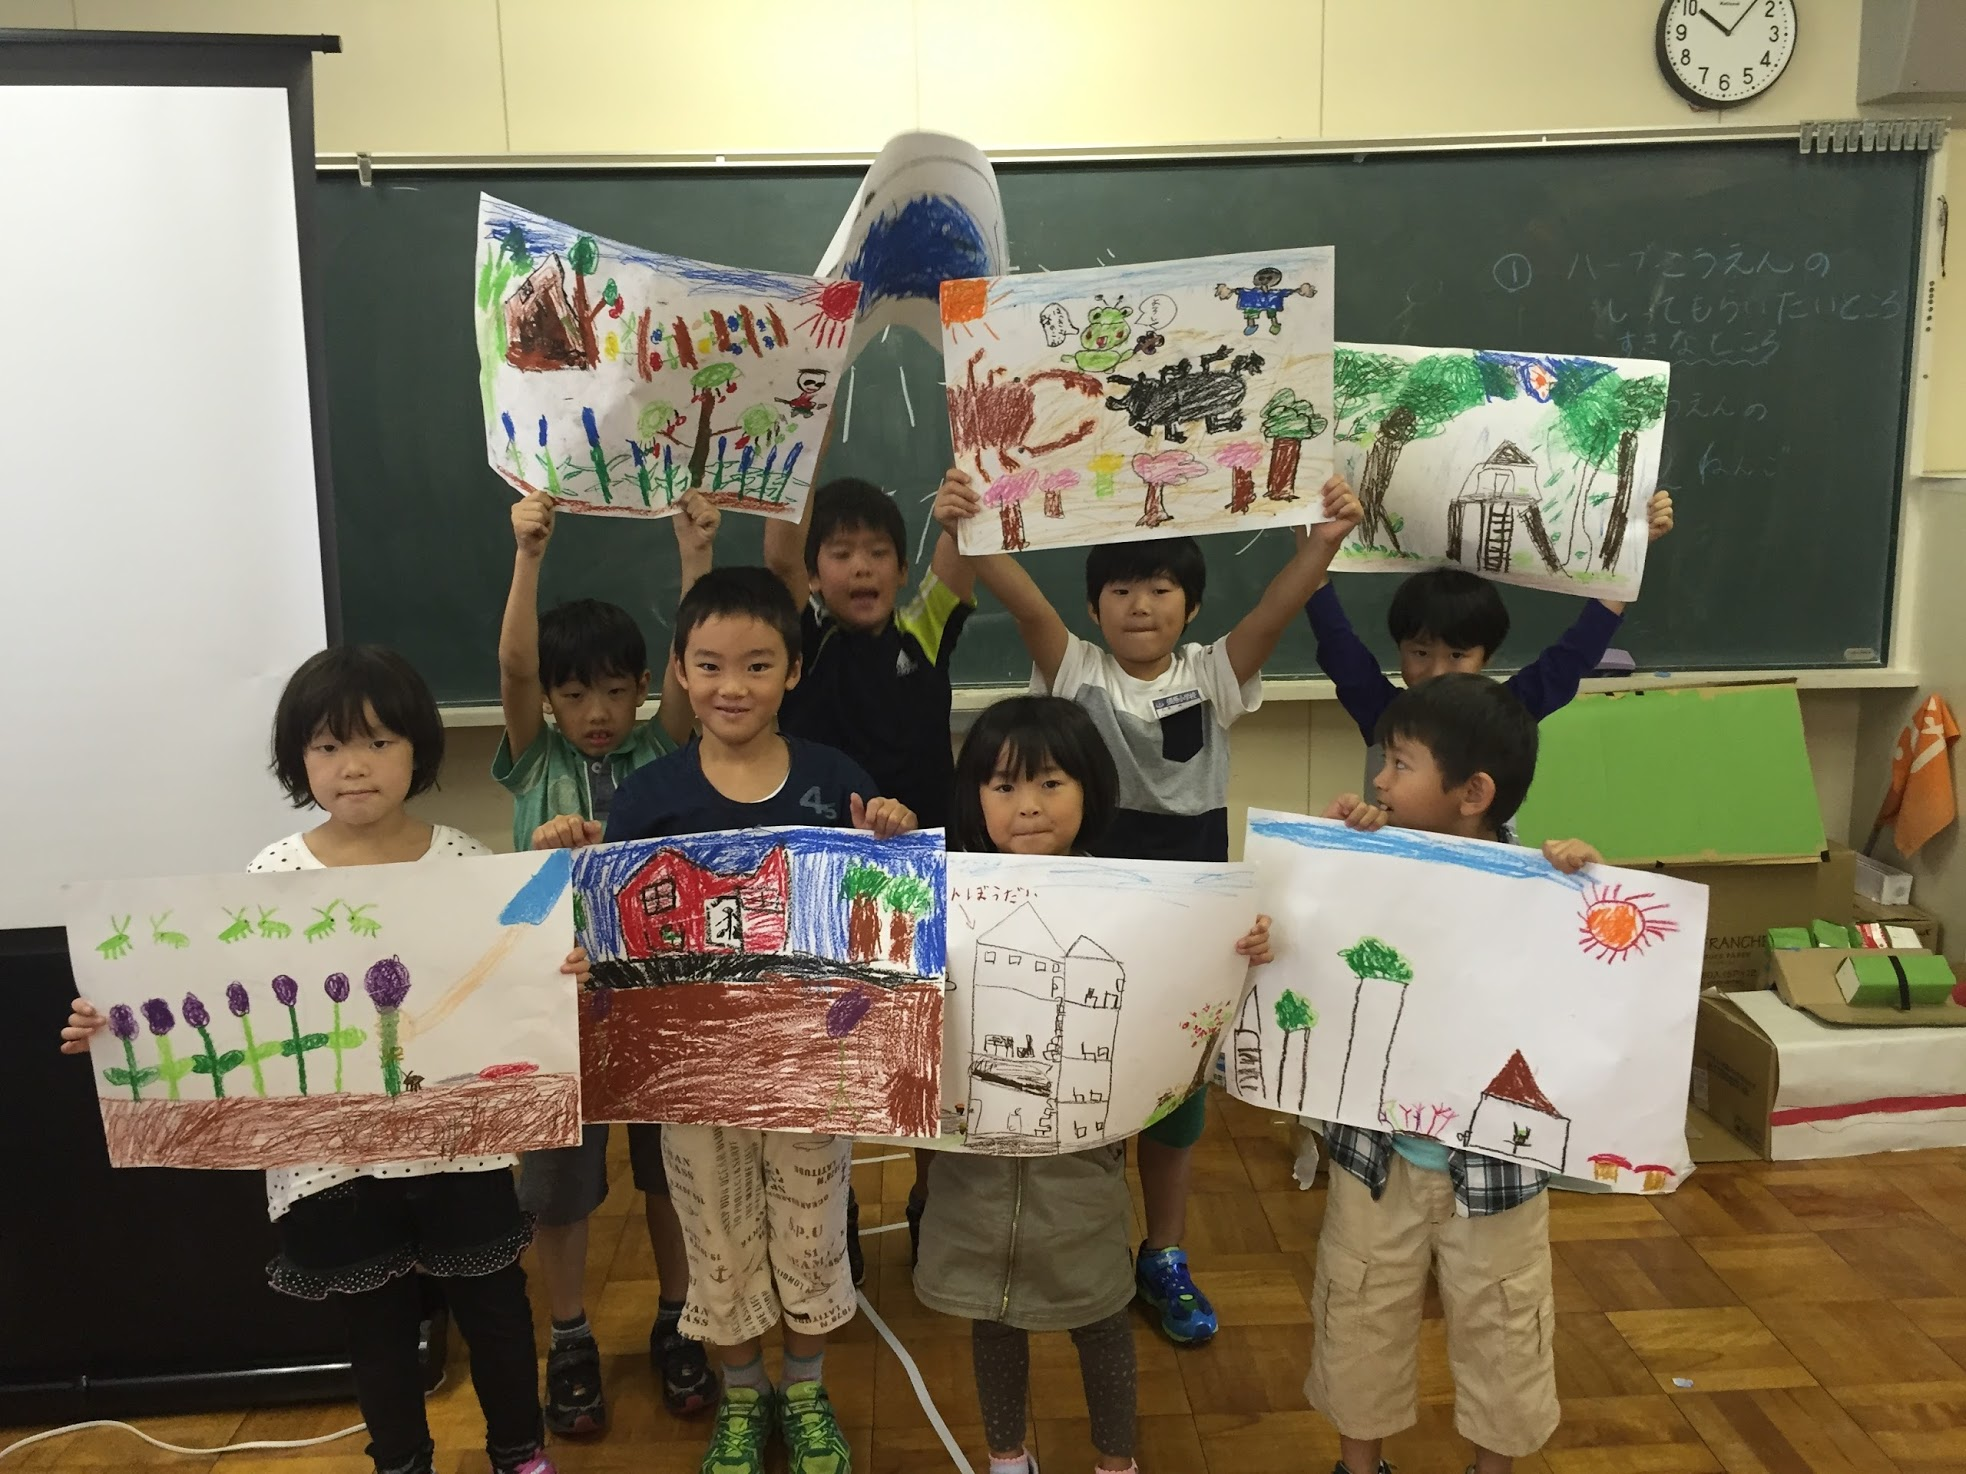
\includegraphics[width=1.0\hsize]{./images/IMG_3723.JPG}
    \caption{成果物1}
    \label{fig:tmu_hino}
  \end{center}
\end{figure}
\begin{figure}[H]
  \begin{center}
    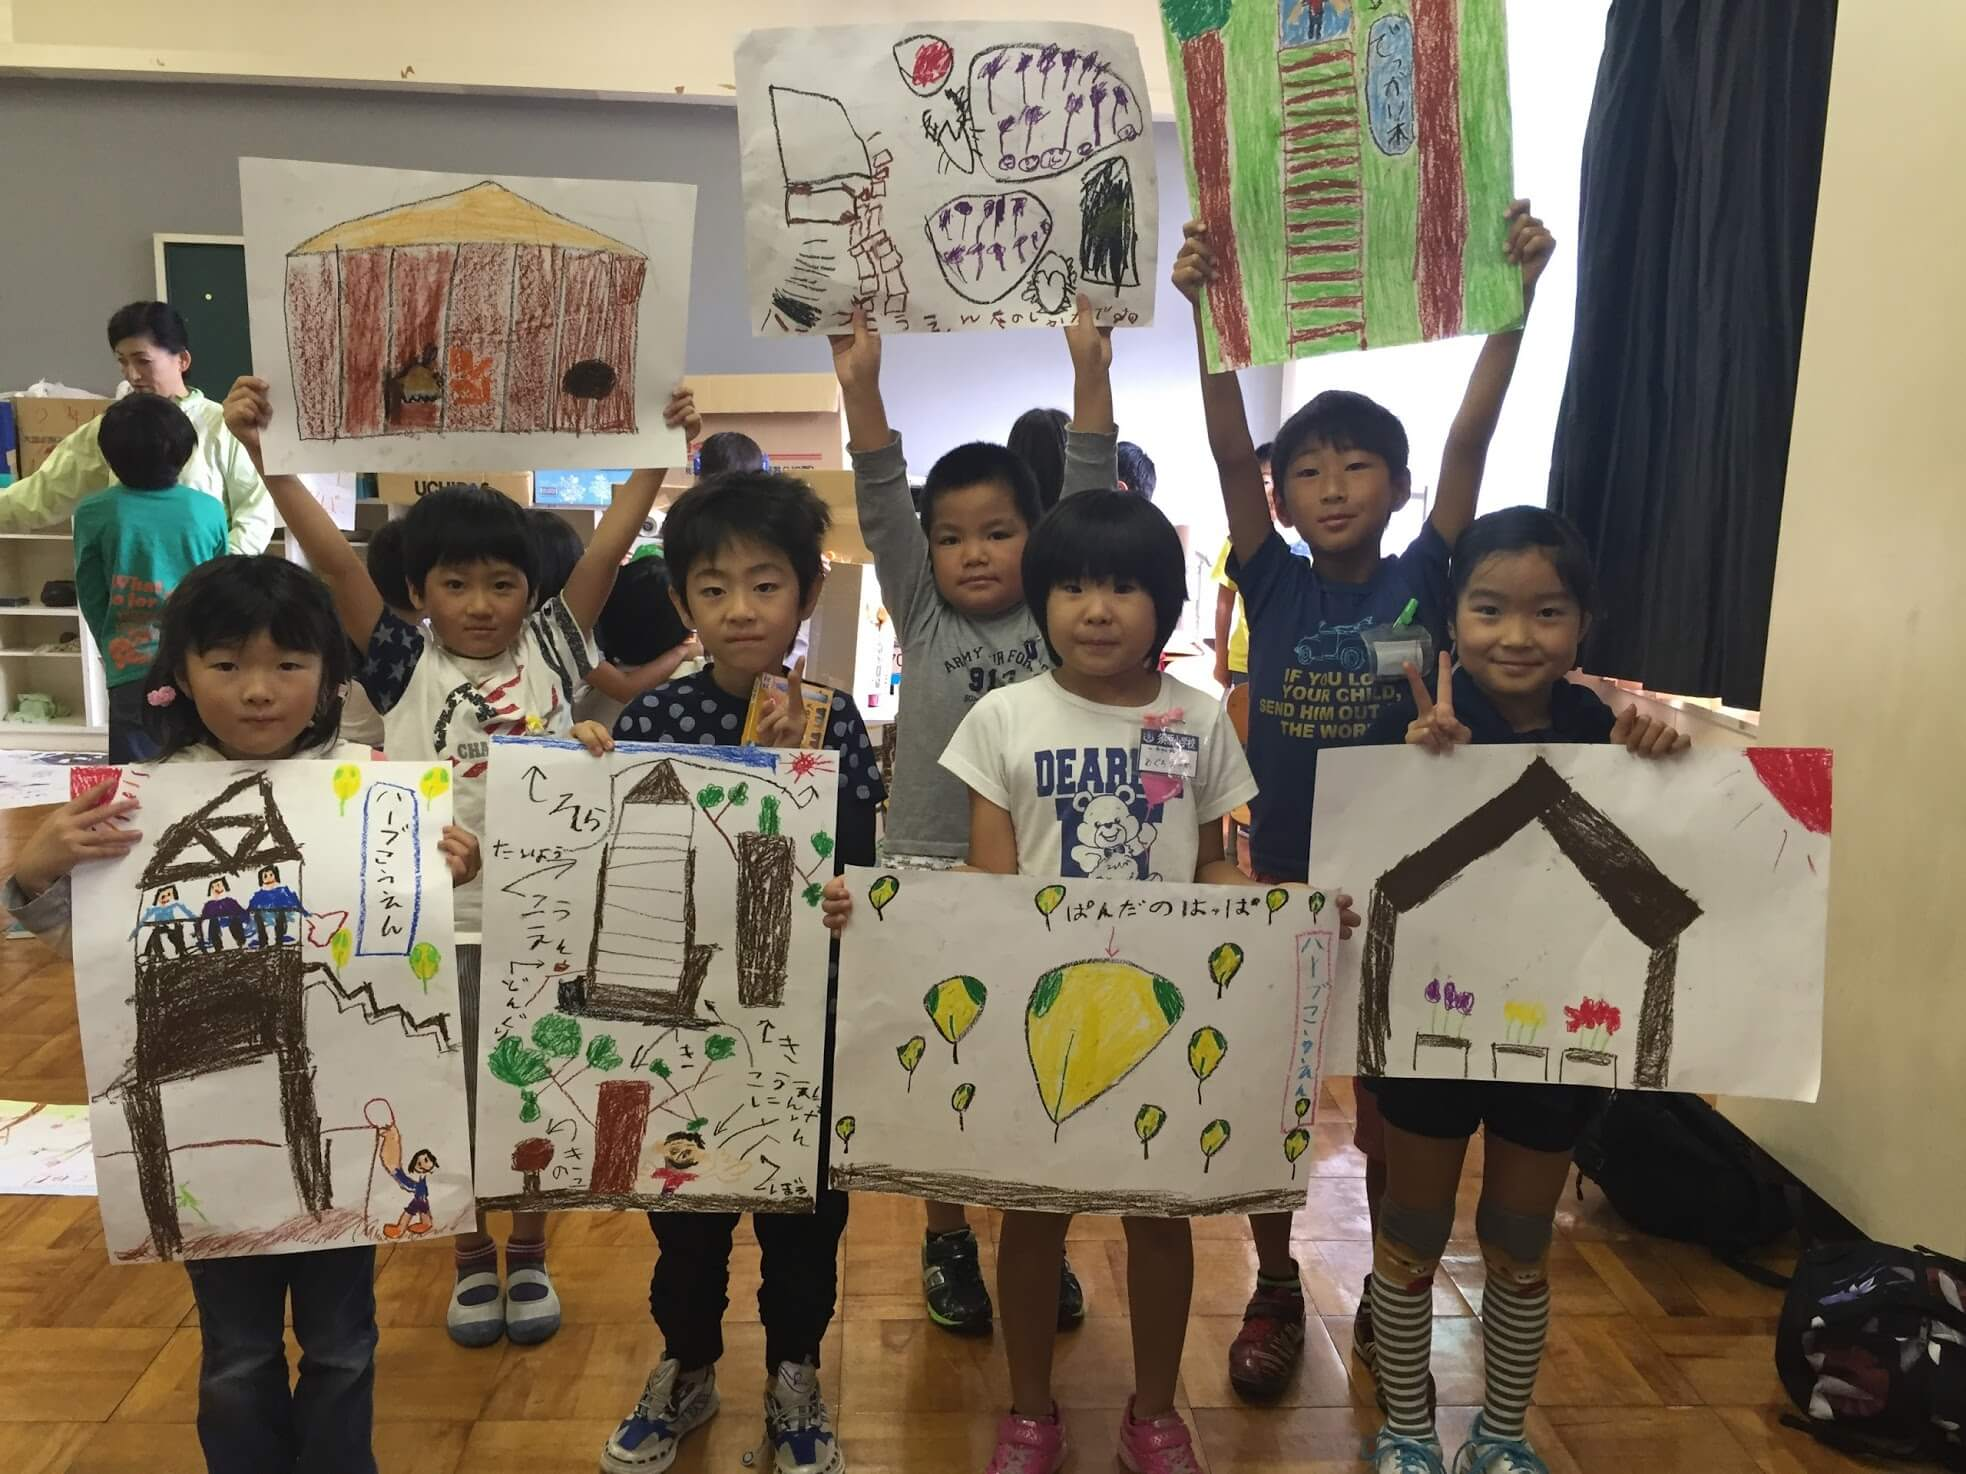
\includegraphics[width=1.0\hsize]{./images/07.jpg}
    \caption{成果物1}
    \label{fig:tmu_hino}
  \end{center}
\end{figure}


上記の二つのワークを元に,動画・冊子の鑑賞できるコンテンツを制作した.これらをプログラム5“食事”時にチームごとにこれらのコンテンツを鑑賞する時間を持つ.かしこまらずに自然体でいる時間帯にコンテンツを起爆剤としておくことで,気張らずに地域の過去・将来についての会話を促進することを企図する.\\\\


\end{itemize}
3-B:[協働作業]:様々な年代のメンバーが参加するチームを編成し,世代を超えた協働作業を行なう.\\\\
会場設営時,机で4つの山を作り,クリスマス会に到着した人から番号を振り,自然に世代がバラバラなチームになるようにする.チームで力を合わせて行う,紙飛行機の飛行距離をきそうゲーム,その勝敗で具材が選べるクリスマスケーキ作りを行う.これによって,世代の違う住民たちが自然にコミュニケーションを取れるように心がける.\\\\

3-C:[自然体]:開催する場所・時間帯を,地域の慣習に合わせることにより,メンバーが気張らず,平常心で参加できるようにする.\\\\
普段から地域行事開催の中心施設となっているみずほ会館を使用し,時間帯も仕事・学校などの関係上,休日の夕方に設定した.\\\\
\subsection{結果}
参加者は,WEBアプリ作成のためのマッピングワークショップの参加者にプラスして,図◉でもわかる通り、小学生を中心とした子供世代・30代女性・50-70代女性の参加が見られ,課題としてあげられた「参加者の世代・性別のばらつき」を抑えることができた.各世代への役割付けに対しては、図◉と図◉の写真からわかるように、子供達がただ参加するだけではなくて使命感をもって生き生きと参加している様子を見ることができた。さらに普段は関わりのない子供と接することで「子供はいいね〜。地域の宝だね〜。」と改めて地域の子供を可愛がる様子も見ることができた。母親世代の料理を作る役割に関しても、料理というコンテンツを介して、世代を超えて「普段はなかなかきけないのよね。」「実は、横根に古くからある〇〇の作り方を誰かおしえてくれないかな〜っておもってたの。」などと、おばあちゃん世代とのコミュニケーションの場になっている姿を見ることができた。
\begin{figure}[H]
  \begin{center}
    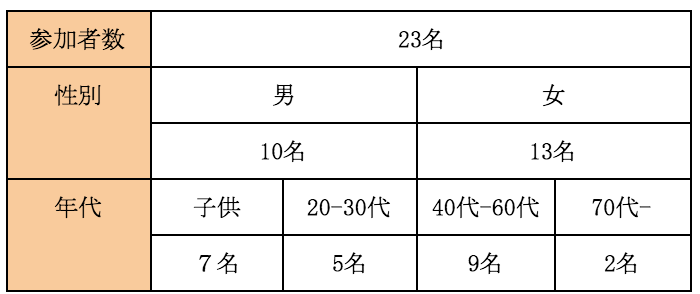
\includegraphics[width=0.7\hsize]{./images/20.png}
    \caption{参加者の属性}
    \label{fig:tmu_hino}
  \end{center}
\end{figure}
\begin{figure}[H]
\begin{center}
  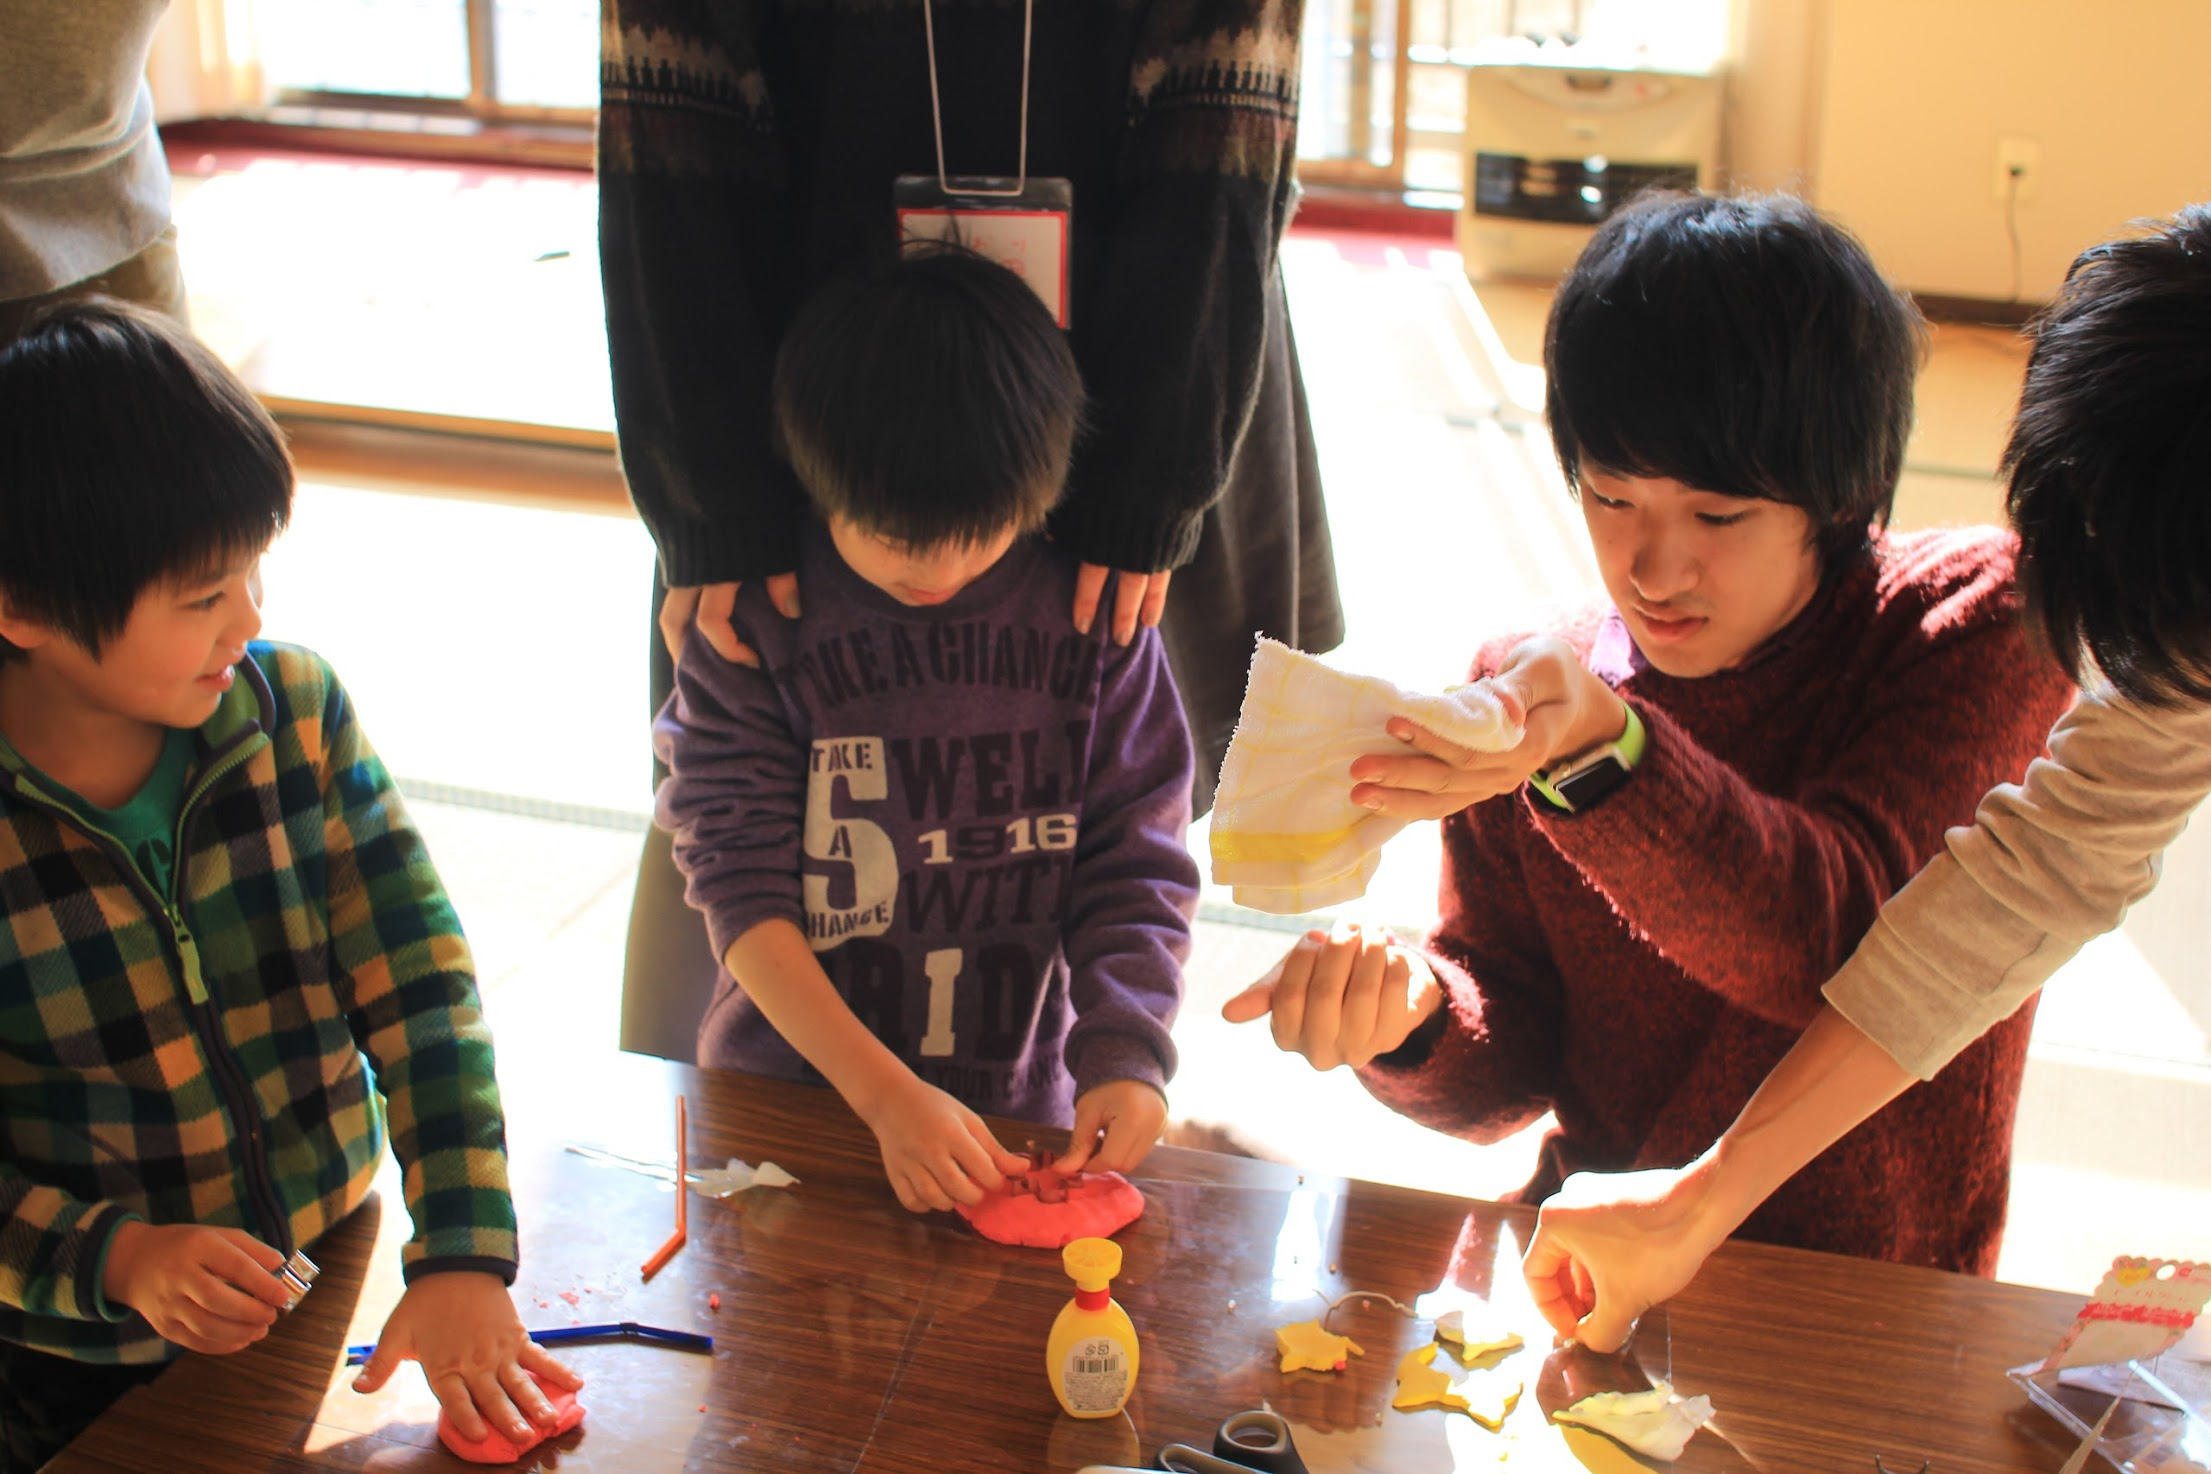
\includegraphics[width=0.95\hsize]{./images/IMG_5929.JPG}
  \caption{子供たちによるプレゼント作成の様子}
  \label{chirstmas2}
\end{center}
\end{figure}

\begin{figure}[H]
\begin{center}
  \includegraphics[width=0.95\hsize]{./images/DSC_0192.JPG}
  \caption{子供たちによるプレゼント配布の様子}
  \label{chirstmas2}
\end{center}
\end{figure}

ゲームや協働作業では,共通に与えたれたミッションを一緒にこなすことで,年齢の壁を超えて力を合わせ自然にコミュニケーションを取れている姿が見られた.さらに,図◉からもわかる通り、協働作業後の仲がほぐれた状況で世代の違う参加者同士が会話促進コンテンツを見ることで「30年前はよく若い衆で集まって旅行や飲み会したんだよ,またやりたいなあ」「20年後は何歳になるの?その頃,横根はどんな風になってるかね」など各世代の目線から集落“横根”についての過去・現在・未来について会話が弾んでいる姿が見ることができた.コンテンツに映る帰省者や親戚の地域に対する意見を聞くことで「たしかにこういうところもいいところだよね」と改めて自分の地域を客観視し,改めて地域愛着を感じている姿も見ることができた.\par

\begin{figure}[H]
  \begin{center}
    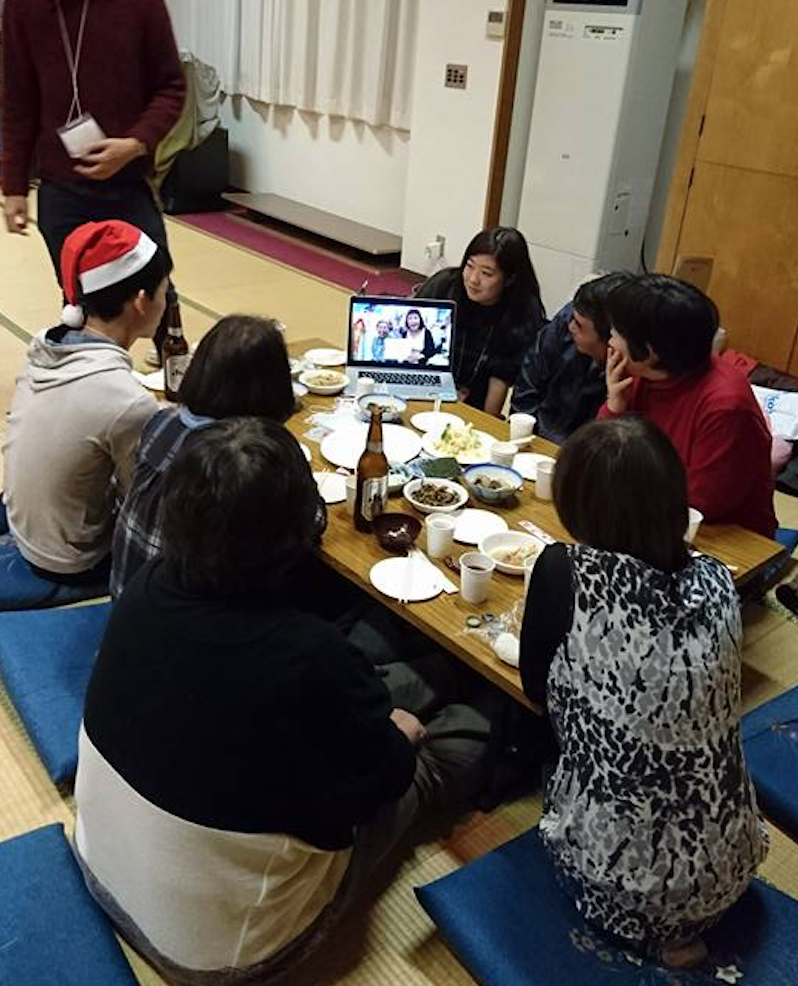
\includegraphics[width=0.6\hsize]{./images/09.png}
    \caption{コンテンツ鑑賞の様子}
    \label{fig:tmu_hino}
  \end{center}
\end{figure}


さらに,これまで地域活動に参加してこなかった50代女性から「人が減ってきて集まりがへってきてたけどもっと開催したいね」「懐かしいな」という声が聞こえ,30代女性からは「自分たちが最後の世代だったけど,子供神輿を子供達に経験させてあげたいな」などという自発的な“場”の提案も見られた.\par
さらに,その後の経過として,この“場”か提案された“子供神輿”について,これまで一緒に協働作業や行事の参加をしていなかった30代女性が50代〜60代の男性である自治構成員世代に協力を仰ぎ,自発的に準備・実行された.図◉からもわかる通り、地域のおじいちゃんが先頭を歩き笛を拭きながら、実行された“子供神輿”は地域の子供だけでなく、お盆で帰省した子供たちも集まっている。お母さんや帰省者、様々な世代性別が集合し見守る姿も見ることができた。(図◉)これは、地域本来の対話と交流の 「場」の 復活である。それに伴い,図◉にもある通り、今まで自治構成員のみで行っていた地域行事「守門祭り」の事前準備に30代女性や子供が自主的に参加する姿なども見ることができた.

\begin{figure}[H]
  \begin{center}
    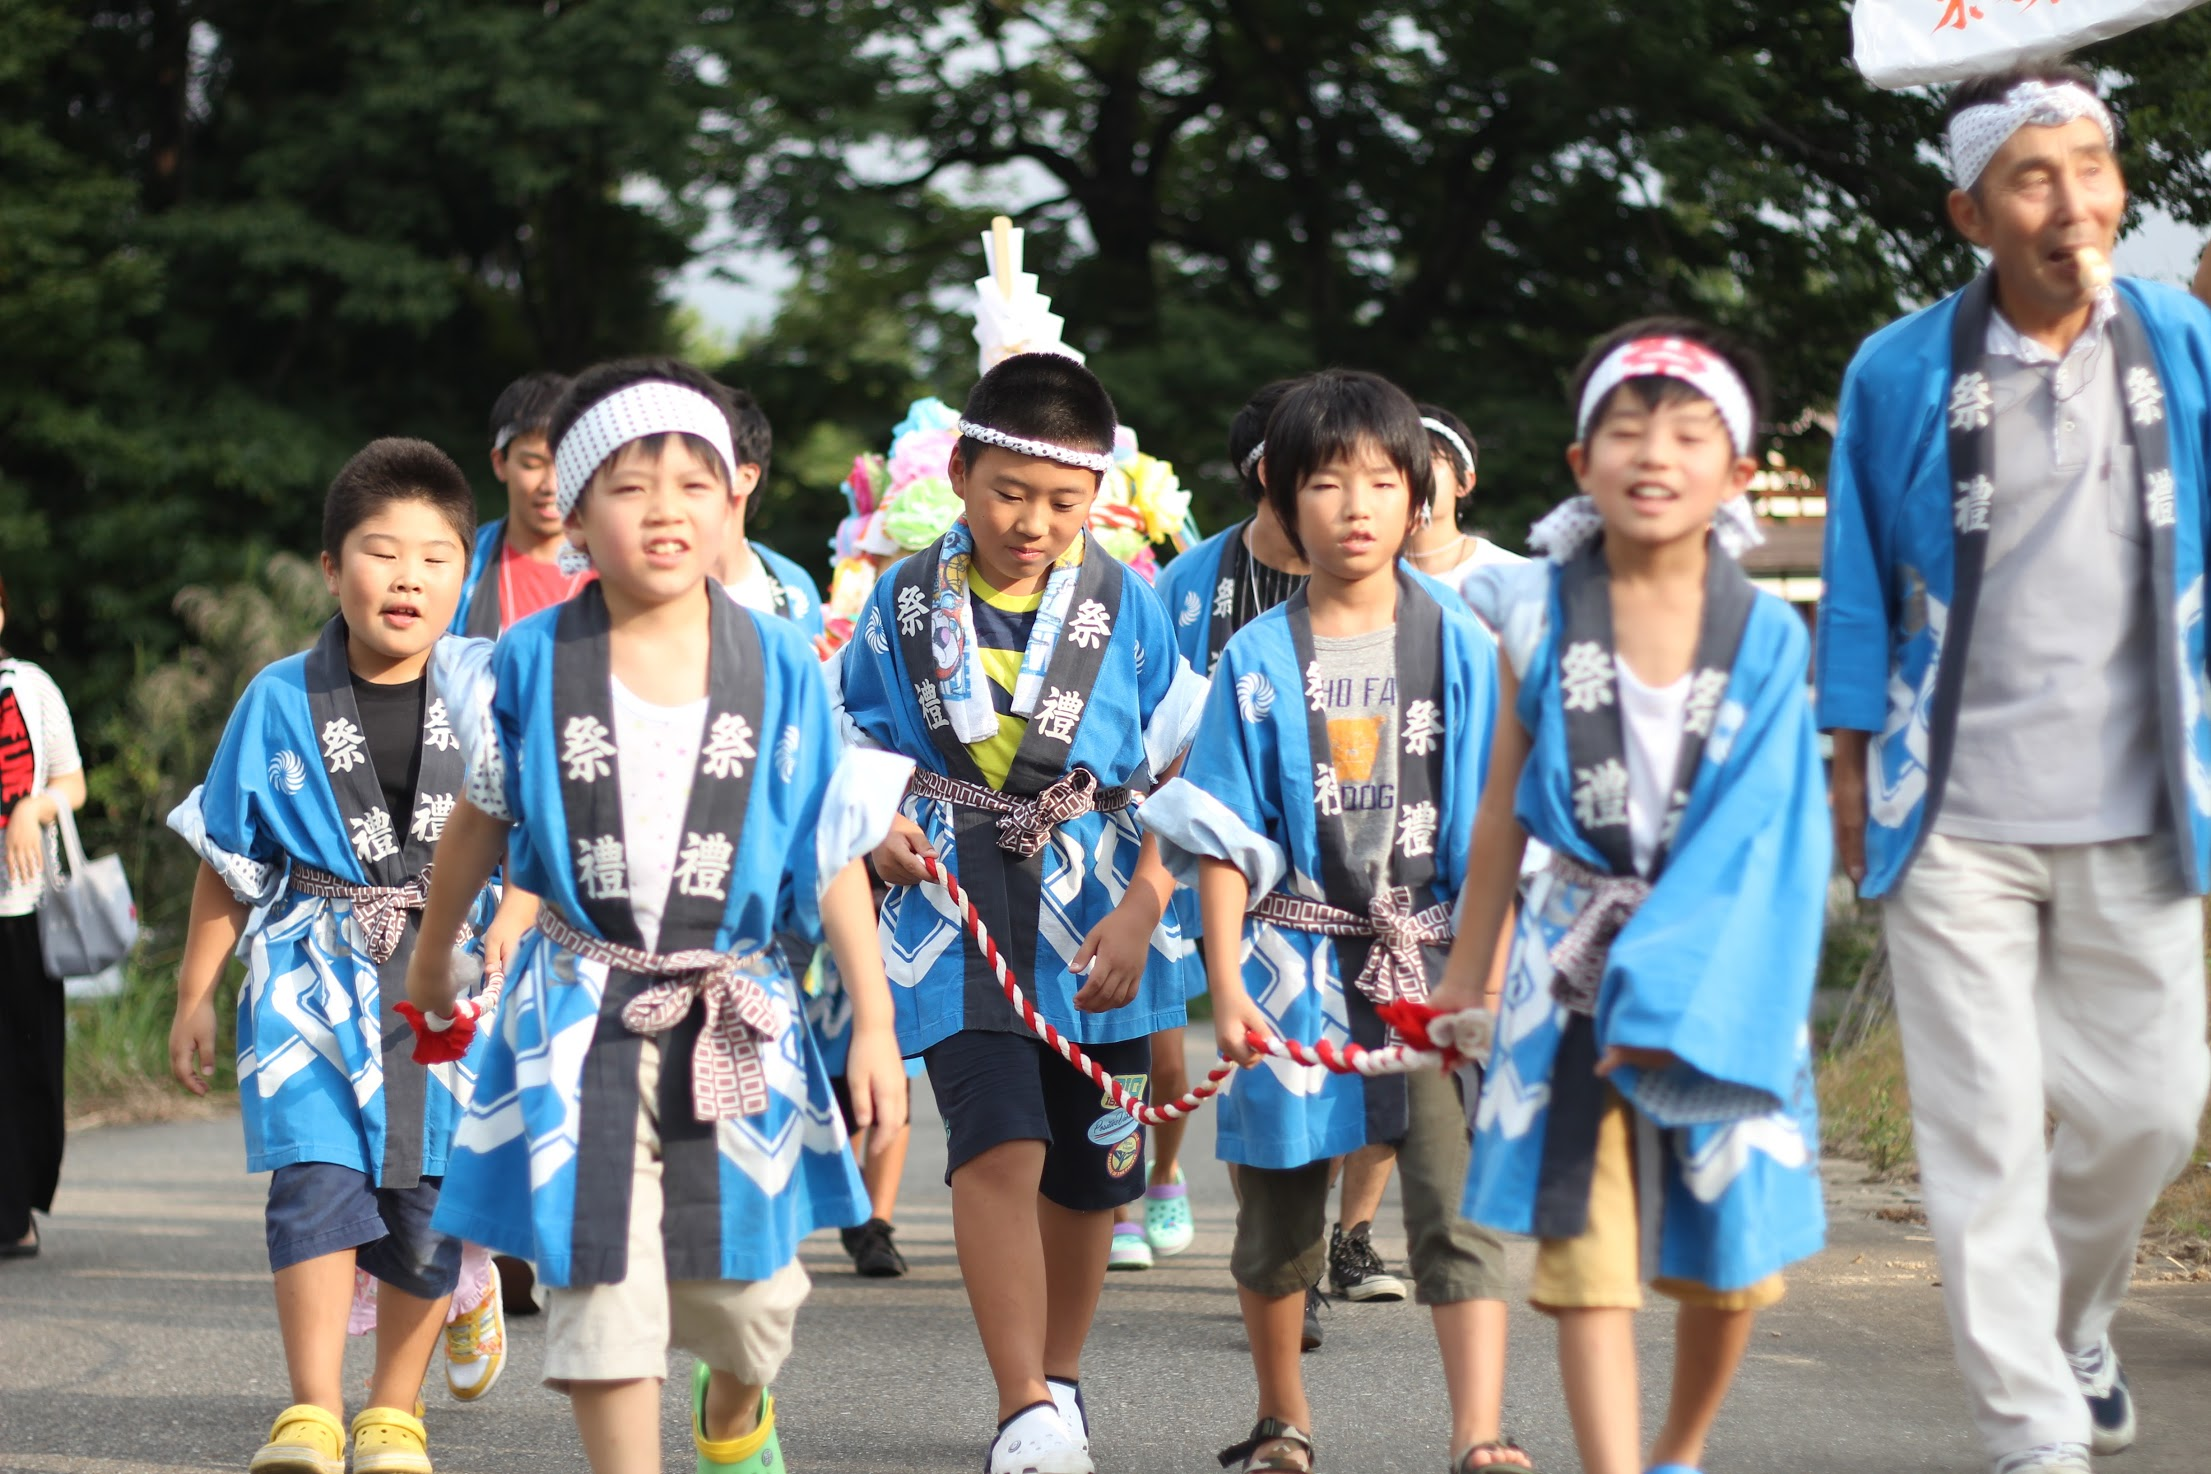
\includegraphics[width=0.9\hsize]{./images/IMG_0744.JPG}}
    \caption{実行された子供神輿の様子}
    \label{fig:tmu_hino}
  \end{center}
\end{figure}\begin{figure}[H]
  \begin{center}
    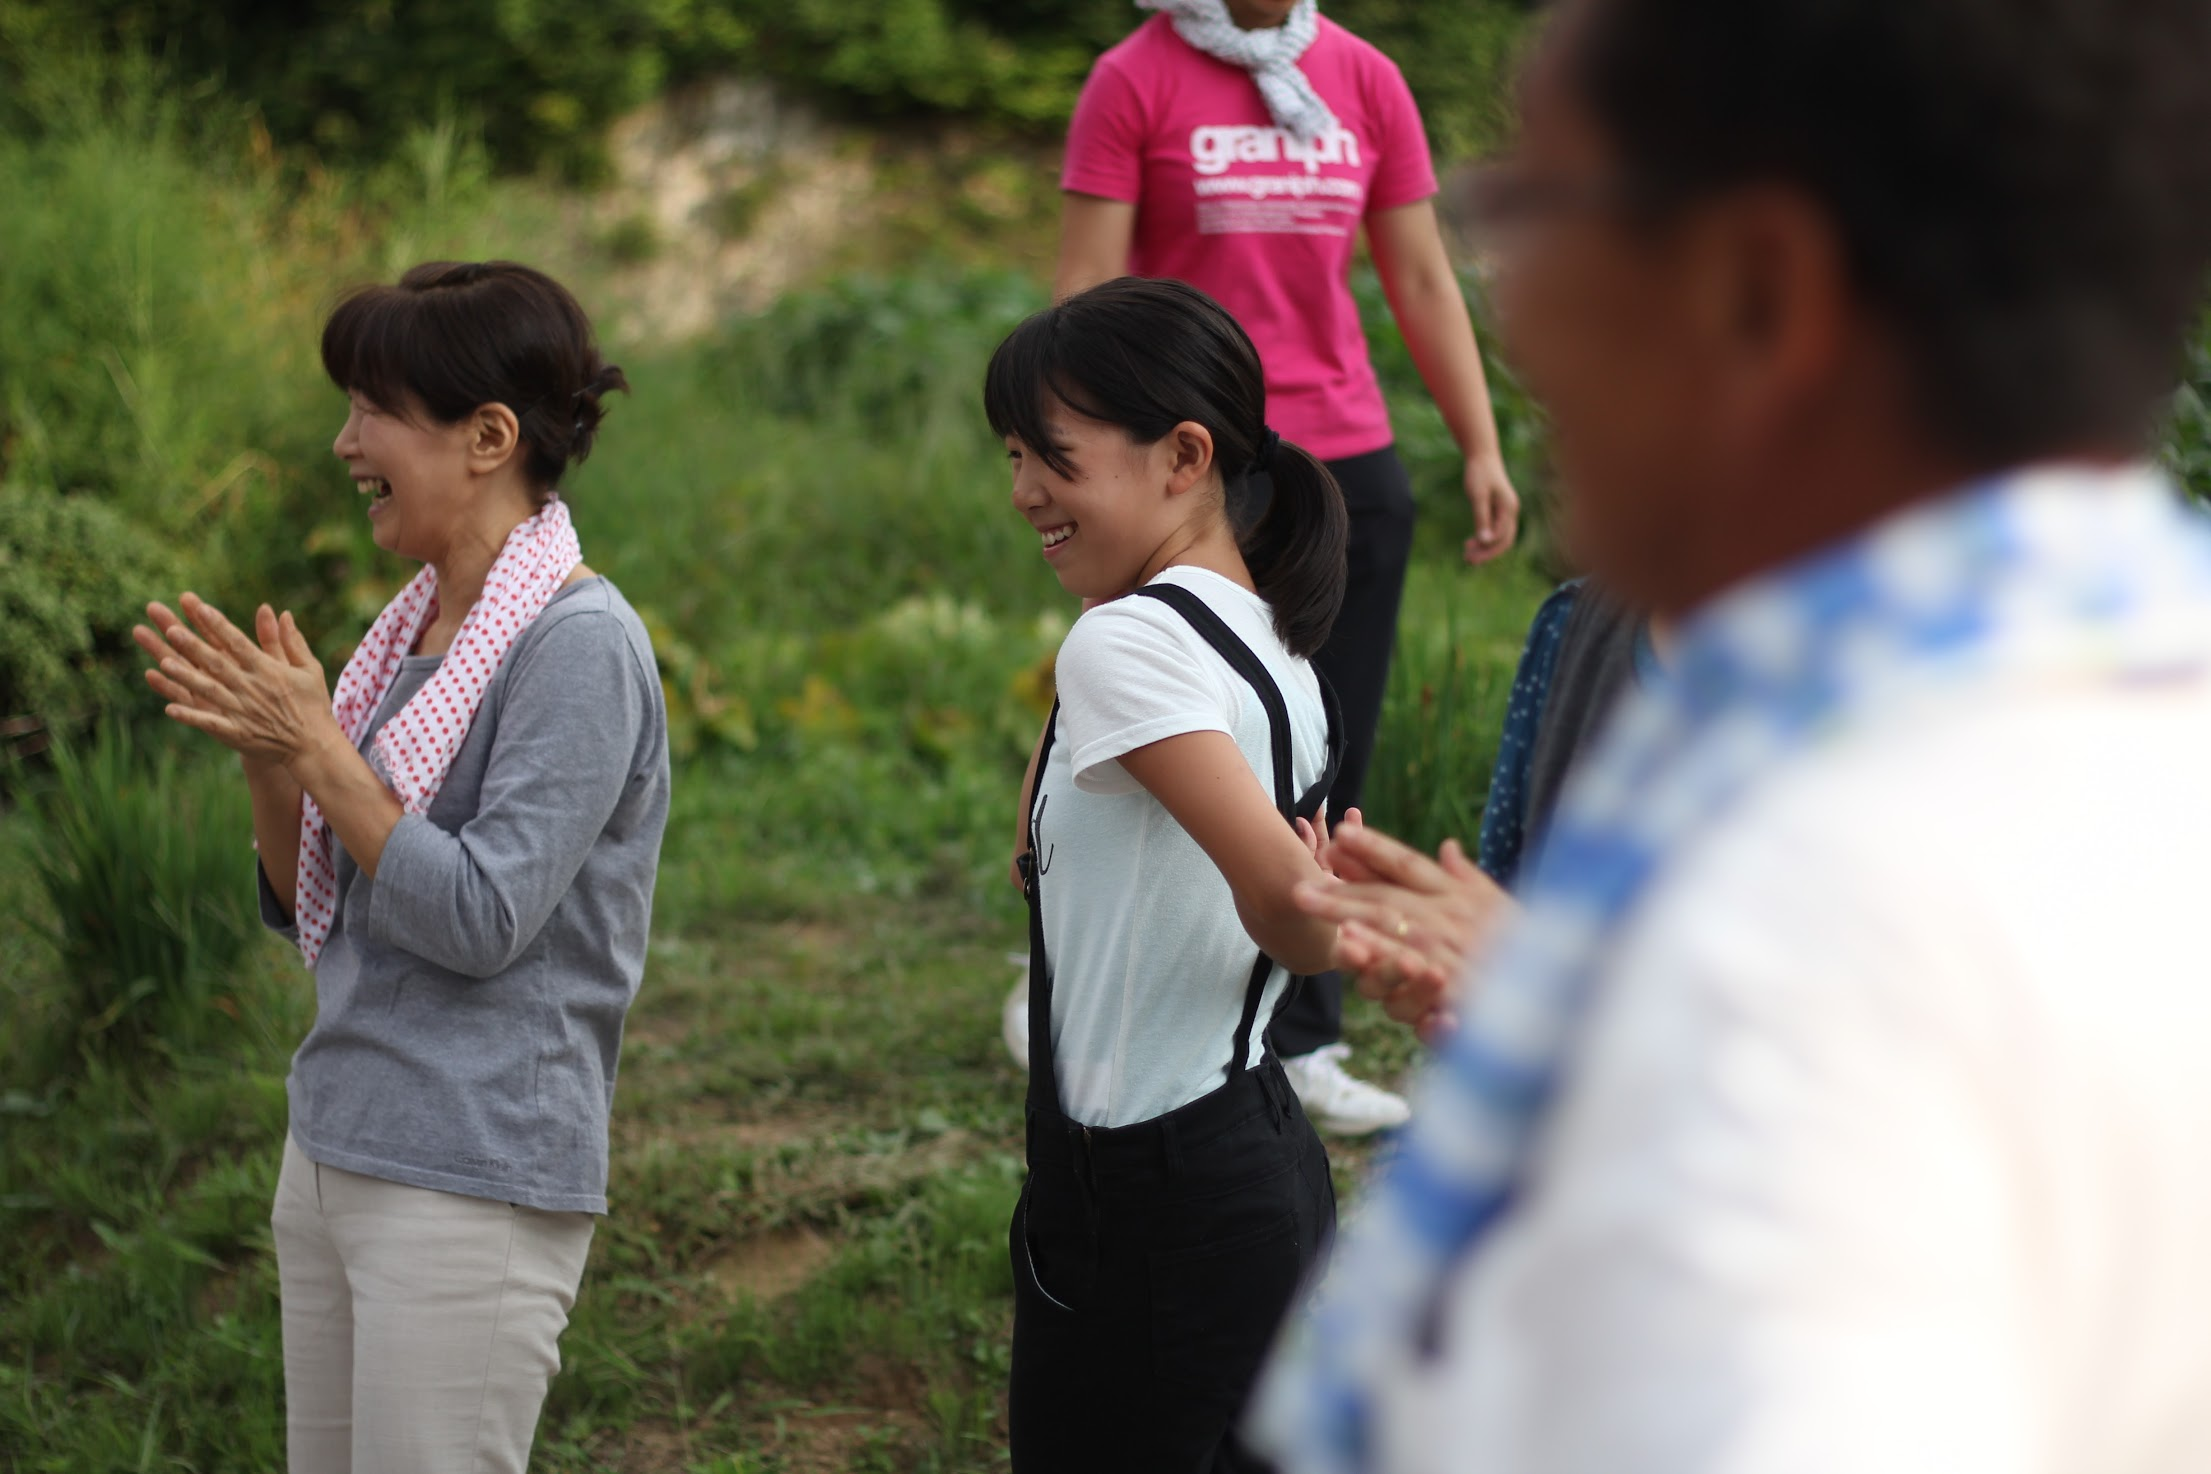
\includegraphics[width=0.9\hsize]{./images/IMG_0747.JPG}
    \caption{見守る地域住民の様子}
    \label{fig:tmu_hino}
  \end{center}
\end{figure}
\begin{figure}[H]
  \begin{center}
    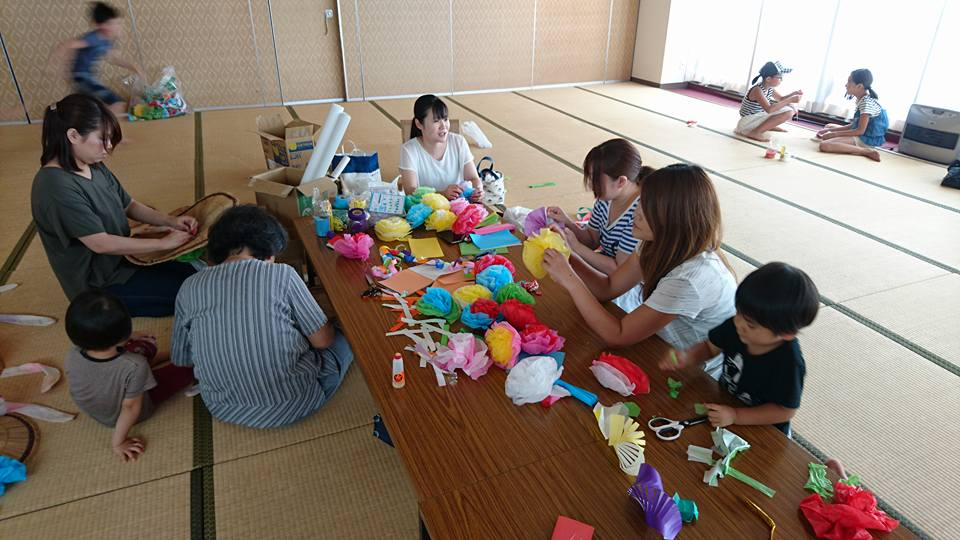
\includegraphics[width=1.0\hsize]{./images/24.jpg}
    \caption{事前準備の様子}
    \label{fig:tmu_hino}
  \end{center}
\end{figure}


\subsection{考察}
これらの結果は,今回用いた「パターン」の組み合わせによって,適切な“場”が形成されたことを示している.従って,筆者の手法は有効なものであるといえる.\par
特に,起爆剤として用意したコンテンツの鑑賞時には,いつもは,発言の少ない人も進んで前向きな地域語りを行っていた.これは直接的ではなく近しい人間の意見を介して地域を考えることがきっかけになり,かしこまることなく自然体で話せていたことが原因であると推測できる.
\par
世代の離れた相手にも,「おばちゃんのことわかる?」「知ってるよ.あの坂の上にすんでるよね」「私のお家はあなたのおじいちゃんにつくってもらったのよ.」などの会話も見られた.人口減少によって“場”が徐々に減ることで,コミュニティーの弱化がみられる横根地区だが,その一方で立地や条件から集落の規模の小ささが特徴でもあり,そもそも近隣住民同士の潜在的なつながりは強い.つまり,適切な“場”をつくることができれば,世代年齢関係なく共通項が多い住民同士の交流は生まれやすい.“場”を形成したことで,その中から自発的に地域行事を復活させようという声が上がり,そこから一気に協力体制が整い,15年間行われていなかった行事が実践された.これは本研究がもたらした効果が単年度に留まらず,継続していく可能性を示していると考えられると同時に,地域住民が集まり交流する“場”をつくることが過疎地域においていかに重要であるかを示している.\par
地域住民だけではなく,近隣集落や地域関係者を巻き込んだ起爆剤コンテンツを介すことで他の人の地域への思いを知り,改めて自分自身が地域について客観的に考える機会になっていた.さらに子供や地域外の人間(スタッフとして入った学生)に「昔はこうだったんだ」「冬はこんなになるんだよ」などといった地域語りも数多く見られた.これは“場”における“よそもの”や“わかもの”などの異分子の重要性を示してると考えられる.\par
さらに,その後のヒアリングで「地域のために,今動かないと手遅れになる.いまはまだ考えているだけだけど,何かしたいなって最近思うようになった.」という声が聞くことができた.これは地域再生に向けた地域住民のモチベーション(活性化の意図)の萌芽とその高まりや連鎖(活動の創発)を生んだと言える.つまり,“場”は地域に改めて愛着を感じる機会を形成するだけではなく,それと同時に長谷川ら[13]が支持する"地域活力向上のサイクル”である地域の現状把握(意識化)から問題意識に膨らませ(問題化),そこから理想的な状態(願望)に向けて目指すべき方向性(目標)を定めて行動を起こして,その結果満足感が得られれば次なる問題意識が芽生え,サイクル的に地域活性化が図られる”(図〇〇)における,“意識化”への導入にもなるとも言えるだろう.

\begin{figure}[H]
  \begin{center}
    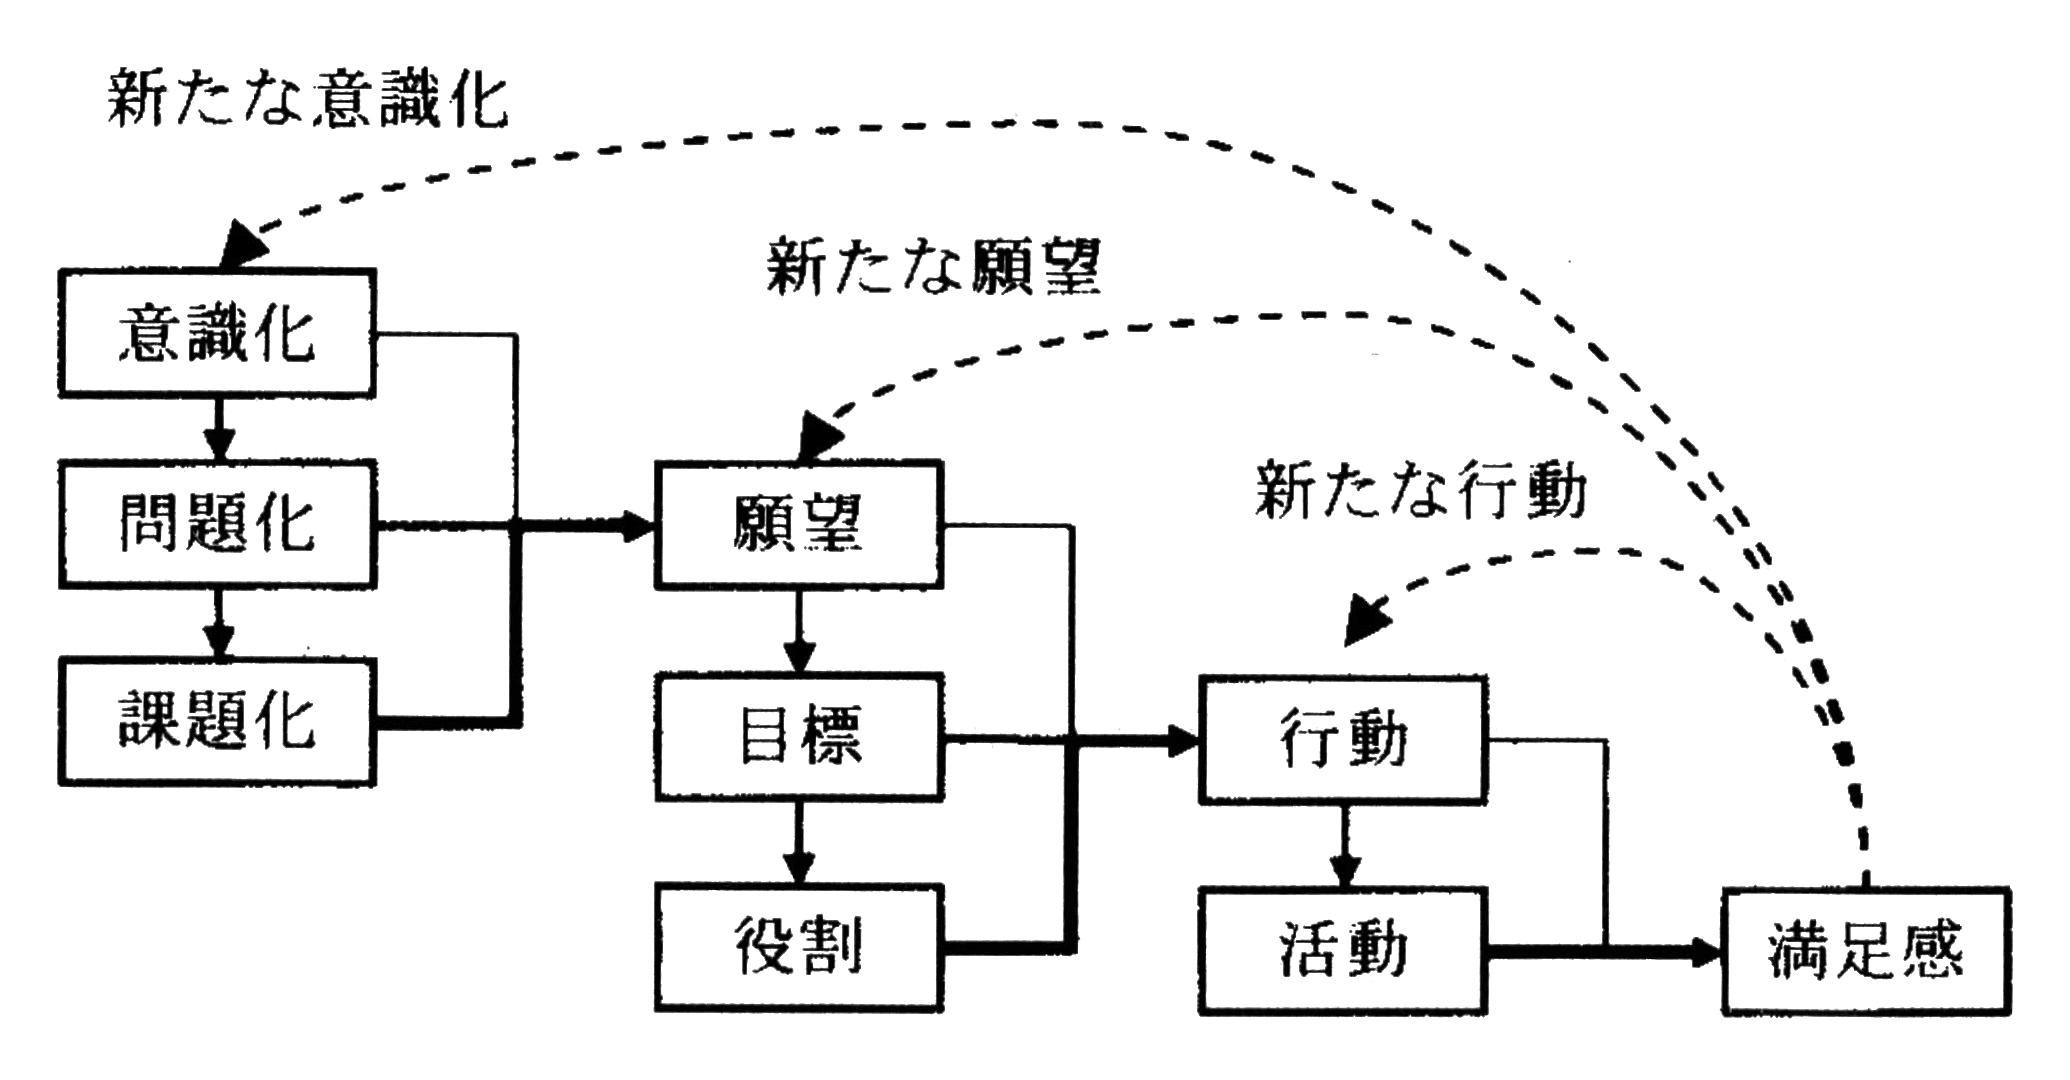
\includegraphics[width=1.0\hsize]{./images/16.jpg}
    \caption{地域活力向上のサイクル(参照:長谷川ら[13])}
    \label{fig:tmu_hino}
  \end{center}
\end{figure}

\newpage
\section{まとめ}
本研究の結論および研究成果が持つ意義を述べる.新たな問題点や展望をまとめる.

\subsection{本研究の概要と成果}

本研究では,集落組織が弱体化した過疎地域における「対話と交流の“場”」を形成する手法について検討することを目的に,新潟県魚沼市の過疎地域である横根地区を対象地域とし,同地域で行われたワークショップを“場”の形成の面から考察.課題点をもとに過疎地域における“場”の設計・運営のガイドライン及びパターンにまとめ,それをもとに“場”を実践することでその有効性を示すことができた.\par
さらに,“場”の形成とともにその後の地域活性化の経緯を見守ることで,地域おこし協力隊や大学生などの“よそもの”の協力などを得ながら,新たな地域活動への意欲形成などの内発的発展の流れを読み取ることができた.\par
本研究の意義は,社会における重要な課題となりつつある「限界集落の地域活性化」のありかたについて,住民の地域主体性とシビックプライドの見地から再検討し,さらに実際の集落における「対話と交流の“場”」づくりの実践を通して,その有効性を示したことである.本研究の成果は,専門家でなくとも利用可能であり,今後国内に増えていくと予想される限界集落における諸問題を解決するための,一つのモデルとなりうると考える.


\subsection{今後の課題と展望}
山下らが「集落の人々が主体的に取り組む気持ちの涵養が重要視され,集落に居住していない人々,その地の出身者や近くの集落,また中心都市の人々も,集落に積極的に関わらせていく必要がある」\cite{7}と論じているいるように、過疎集落は、次のステップとして地域出身者や地域訪問者などの地域関係者への地域外コミュニティーの拡張が必要である。

本研究において“場”の企画・運営は,主に東京に住む地域外のスタッフが担った.実践の前にスタッフが継続的に集落に通い,田植え・稲刈りなどの地域地場産業の体験やお祭りなどの地域伝統行事の参加など集落との信頼関係を築いたのも成果の要因でもあると考えられる.これには最低限の期間と予算が必要となる.初年度こそ新潟県からの助成金事業で行ったが,次年からは,活動費の調達が難航した.次年度は研究室の研究費や市からの助成での補填,三年目はGakuvo(日本財団による学生ボランティア助成)・大学同窓会の学生活動助成によって補填され活動を行った.“場”の形成において,地域外の人間,いわゆる“よそもの”の存在の重要性が示された一方で,“よそもの”の確保・継続的な派遣に伴う予算の獲得も一つの課題である.\par


\newpage
\section*{謝辞}
\par
本論文は筆者が首都大学東京大学院システムデザイン研究科インダストリアルアート学域博士前期課程に在籍中の研究成果をまとめたものです.
\par
本研究におよび本論文の執筆において,多くの方々からご指導やご支援をいただきました.この場を借りしてお世話になりました方々に厚く御礼申し上げます.
\par
本研究を進めるにあたり,指導教官として本研究の実施の機会を与えて戴き,その遂行にあたって終始,ご指導やご助言をいただきました,渡邉英徳先生に謹んで感謝の意を表します.
また,今間俊博先生,並びに,難波治先生には副査としてご助言を戴くとともに本論文の細部にわたりご指導を戴き,ここに深く感謝の意を表します.
\par
横根集落の活動にあたり,ご尽力いただきました魚沼市の佐藤陽二さん,魚沼市地域おこし協力隊の大野久美子さんにも深く御礼申し上げます.
\par
最後に,本研究を支え,日常の議論を通じて多くの知識や示唆を頂いたネットワークデザインスタジオのみなさんに深く感謝致します.
\newpage
\begin{thebibliography}{999}


\bibitem{2}国土交通省重点政策(2016)、<http://www.mlit.go.jp/common/001143046.pdf>2016/06/02更新,2016/07/14参照
\bibitem{3}
安藤生恒,(1981),『過疎地再生の道』,日本経済評論社 pp.88~98
\bibitem{4}
長谷川・藤沢・竹本・荒樋,(1996),『過疎地域の景観と集団』,日本経済評論社 pp.20~28
\bibitem{5}山下祐介,(2012),『限界集落の真実 ―過疎の村は消えるか?』,ちくま新書 p.19-40
\bibitem{6}土居 洋平,(2008),『「地域コミュニティ問題」の現状と課題』共済総研レポートp.6
\bibitem{kasseika}、(2014)、「地域活性化の定義・分析手法等について」、農林水産省、p3-28
\bibitem{arek}クリストファー・アレグザンダー、(1984)、『パタン・ランゲージ:環境設計の手引』 鹿島出版会,
\bibitem{ptn}井庭崇、(2011)、『パターンランゲージ 3.0』,情報処理vol.52 No9,p1151−1156
\bibitem{a}安藤生恒,(1981),『過疎地再生の道』,日本経済評論社 pp.88-98
\bibitem{shiomi}塩見譲編,(1989),『地域活性化と地域経営』,学陽書房 p.253
\bibitem{7}鈴木春菜,(2008),『地域愛着が地域への協力行動に及ぼす影響に関する研究』,土木計画学研究・論文集 25(2).p357-362
\bibitem{8}清水博編著 (2000) 「場と共創」 NTT 出版や清水博 (2003) 「場の思想」 東京大学出版会
\bibitem{9}伊丹敬之 (2005) 「場の論理とマネジメント」 東洋経済新報社
\bibitem{10}和田崇編 (2005) 「創発まちづくり~動く・繋がる・生まれる」 学芸出版社 対話と交流の場づくりから始めるまちづくりのあり方に関する一考察 45
\bibitem{11}久隆浩 (2008) 「景観づくりはまちづくりから」 都市問題研究, 第60巻 第5号, p.74-85, 都市問題 研究会
\bibitem{12}浅海義治・伊藤雅春・狩野三枝(1993) 「参加のデザイン道具箱」世田谷まちづくりセンターや浅海義治・大戸徹・中里京子(1996) 「参加のデザイン道具箱Part-2 プロセスデザイン」世田谷まちづくりセンター
\bibitem{13}世古一穂(2009) 「参加と協働のデザイン~NPO・行政・企業の役割を再考する」学芸出版社
\bibitem{14}伊藤雅春・大久手計画工房 (2003) 「参加するまちづくり~ワークショップがわかる本」 農文協
\bibitem{15}菊本有紀(2015)「地域住民の参加によるウェブコンテンツ制作を通した継続的な地域活性化促進」
\bibitem{16}久隆浩 (2010) 「都市計画のパラダイムシフト」 都市計画, 第 283 号, pp. 5-10, 日本都市計画学会


\end{thebibliography}

\newpage


\end{document}
